\section{บทที่ 3 การวิเคราะห์เวกเตอร์สำหรับงานวิศวกรรมไฟฟ้า}

\textbf{ชื่อบทภาษาอังกฤษ:} Vector Analysis for Electrical Engineering\\
\textbf{รายวิชา:} คณิตศาสตร์วิศวกรรมไฟฟ้า (Electrical Engineering Mathematics)\\
\textbf{รหัสวิชา:} 5571102\\
\textbf{สาขาวิชา:} เทคโนโลยีวิศวกรรมไฟฟ้า\\
\textbf{คณะ:} เทคโนโลยีอุตสาหกรรม\\
\textbf{ภาคเรียนที่:} 1\\
\textbf{ปีการศึกษา:} 2569\\
\textbf{ระดับผู้เรียน:} นักศึกษาระดับปริญญาตรี\\
\textbf{จำนวนชั่วโมง:} บรรยายและกิจกรรมในชั้นเรียนรวม 6 ชั่วโมง\\

\subsection{1. แนวคิดสำคัญของบท}

ปริมาณทางวิศวกรรมไฟฟ้าหลายชนิดไม่สามารถอธิบายได้ครบถ้วนด้วยค่าตัวเลขเพียงค่าเดียว เนื่องจากต้องระบุทั้ง \textbf{ขนาด} และ \textbf{ทิศทาง} ตัวอย่างสำคัญ ได้แก่ สนามไฟฟ้า ความหนาแน่นฟลักซ์ไฟฟ้า สนามแม่เหล็ก ความหนาแน่นฟลักซ์แม่เหล็ก แรงลอเรนซ์ และความหนาแน่นกระแส การวิเคราะห์เวกเตอร์จึงเป็นภาษาทางคณิตศาสตร์ที่ใช้แทน อธิบาย และเชื่อมโยงปริมาณเหล่านี้ในอวกาศ

บทนี้เริ่มจากความแตกต่างระหว่างสเกลาร์และเวกเตอร์ การแทนเวกเตอร์ในระบบพิกัดฉาก ทรงกระบอก และทรงกลม การดำเนินการพื้นฐาน ดอตโปรดักต์ และครอสโปรดักต์ จากนั้นพัฒนาไปสู่แนวคิดของสนามสเกลาร์และสนามเวกเตอร์ ตัวดำเนินการเดล เกรเดียนต์ ไดเวอร์เจนซ์ และเคิร์ล รวมถึงอินทิกรัลเส้น อินทิกรัลพื้นผิว และอินทิกรัลปริมาตรที่จำเป็นต่อการตีความกฎพื้นฐานของสนามแม่เหล็กไฟฟ้า

สาระสำคัญไม่ได้อยู่เพียงการจำสูตร แต่คือการเลือกเครื่องมือให้เหมาะกับลักษณะทางกายภาพของปัญหา เช่น ใช้ดอตโปรดักต์เมื่อพิจารณาองค์ประกอบตามทิศหรือฟลักซ์ ใช้ครอสโปรดักต์เมื่อพิจารณาแรงที่ตั้งฉากกับความเร็วและสนามแม่เหล็ก ใช้เกรเดียนต์เพื่อหาทิศทางที่ศักย์เปลี่ยนแปลงเร็วที่สุด ใช้ไดเวอร์เจนซ์เพื่อบอกความเป็นแหล่งกำเนิดหรือแหล่งดูดของสนาม และใช้เคิร์ลเพื่อบอกแนวโน้มการหมุนวนเฉพาะที่ของสนาม

\subsection{2. ความรู้พื้นฐานก่อนเรียน}

ก่อนเรียนบทนี้ นักศึกษาควรมีความรู้และทักษะต่อไปนี้

\begin{enumerate}
\item พีชคณิตพื้นฐาน การแก้สมการ และการจัดรูปนิพจน์
\item ตรีโกณมิติ มุมเรเดียน และความสัมพันธ์ของไซน์--โคไซน์
\item เรขาคณิตวิเคราะห์ในระนาบและอวกาศสามมิติ
\item อนุพันธ์ย่อยและอินทิกรัลเบื้องต้น
\item หน่วยเอสไอและสัญกรณ์วิศวกรรม เช่น k, m, \(\mu\), n
\item ความหมายเบื้องต้นของประจุไฟฟ้า กระแสไฟฟ้า แรงดันไฟฟ้า และสนามแม่เหล็ก
\item การใช้เครื่องคิดเลขวิทยาศาสตร์หรือโปรแกรมคำนวณพื้นฐาน
\end{enumerate}

%\begin{quote}
%\textbf{ข้อเสนอแนะก่อนเริ่มบท:} ผู้สอนควรใช้เวลา 10--15 นาทีทบทวนการหาความยาวของเส้นตรงในสามมิติ การหาอนุพันธ์ย่อย และกฎมือขวา เพื่อช่วยลดภาระทางความคิดในช่วงเรียนครอสโปรดักต์และเคิร์ล
%\end{quote}

\subsection{3. คำสำคัญประจำบท}

\begin{table}[htbp]
    \centering
    \begin{tabularx}{\textwidth}{L{0.22\textwidth} L{0.25\textwidth} Y}
        \hline
        \textbf{คำศัพท์ภาษาไทย} & \textbf{คำศัพท์ภาษาอังกฤษ} & \textbf{ความหมายโดยย่อ} \\
        \hline
        สเกลาร์ & Scalar & ปริมาณที่กำหนดด้วยขนาดเพียงอย่างเดียว \\
        เวกเตอร์ & Vector & ปริมาณที่มีทั้งขนาดและทิศทาง \\
        เวกเตอร์หนึ่งหน่วย & Unit Vector & เวกเตอร์ขนาดหนึ่งที่ใช้ระบุทิศทาง \\
        องค์ประกอบเวกเตอร์ & Vector Component & ส่วนของเวกเตอร์ตามแกนหรือทิศที่กำหนด \\
        ระบบพิกัดฉาก & Cartesian Coordinate System & ระบบพิกัดที่ใช้แกน \(x,y,z\) ตั้งฉากกัน \\
        ระบบพิกัดทรงกระบอก & Cylindrical Coordinate System & ระบบพิกัด \((\rho,\phi,z)\) เหมาะกับสมมาตรรอบแกน \\
        ระบบพิกัดทรงกลม & Spherical Coordinate System & ระบบพิกัด \((r,\theta,\phi)\) เหมาะกับสมมาตรรอบจุด \\
        ดอตโปรดักต์ & Dot Product & ผลคูณเวกเตอร์ที่ให้ผลเป็นสเกลาร์ \\
        ครอสโปรดักต์ & Cross Product & ผลคูณเวกเตอร์ที่ให้ผลเป็นเวกเตอร์ตั้งฉาก \\
        สนามสเกลาร์ & Scalar Field & ฟังก์ชันที่ให้ค่าสเกลาร์ ณ ทุกตำแหน่ง \\
        สนามเวกเตอร์ & Vector Field & ฟังก์ชันที่ให้เวกเตอร์ ณ ทุกตำแหน่ง \\
        ตัวดำเนินการเดล & Del Operator / Nabla & ตัวดำเนินการอนุพันธ์เวกเตอร์ เขียนเป็น \(\nabla\) \\
        เกรเดียนต์ & Gradient & เวกเตอร์บอกทิศและอัตราการเพิ่มสูงสุดของสนามสเกลาร์ \\
        ไดเวอร์เจนซ์ & Divergence & สเกลาร์บอกการแผ่ออกหรือรวมเข้าของสนามเวกเตอร์ \\
        เคิร์ล & Curl & เวกเตอร์บอกแนวโน้มการหมุนวนเฉพาะที่ของสนาม \\
        อินทิกรัลเส้น & Line Integral & การรวมปริมาณตามเส้นทาง \\
        ฟลักซ์ & Flux & ปริมาณสนามที่ผ่านพื้นผิว \\
        ทฤษฎีบทไดเวอร์เจนซ์ & Divergence Theorem & เชื่อมฟลักซ์ผ่านผิวปิดกับไดเวอร์เจนซ์ในปริมาตร \\
        ทฤษฎีบทของสโตกส์ & Stokes' Theorem & เชื่อมอินทิกรัลรอบขอบเขตกับเคิร์ลผ่านพื้นผิว \\
        สนามอนุรักษ์ & Conservative Field & สนามที่อินทิกรัลเส้นไม่ขึ้นกับเส้นทาง และมักเขียนเป็นเกรเดียนต์ของศักย์ได้ \\
        แรงลอเรนซ์ & Lorentz Force & แรงต่อประจุจากสนามไฟฟ้าและสนามแม่เหล็ก \\
        \hline
    \end{tabularx}
\end{table}

\subsection{4. ผลลัพธ์การเรียนรู้ประจำบท}

\begin{enumerate}
\item \textbf{อธิบายและจำแนก} ปริมาณสเกลาร์ ปริมาณเวกเตอร์ สนามสเกลาร์ และสนามเวกเตอร์ในบริบทวิศวกรรมไฟฟ้าได้
\item \textbf{เขียนและแปลง} เวกเตอร์ระหว่างระบบพิกัดฉาก ทรงกระบอก และทรงกลมได้อย่างเหมาะสมกับสมมาตรของปัญหา
\item \textbf{คำนวณ} การบวก ลบ ขนาด เวกเตอร์หนึ่งหน่วย ดอตโปรดักต์ และครอสโปรดักต์ พร้อมตีความหมายทางเรขาคณิตและทางกายภาพได้
\item \textbf{วิเคราะห์} สนามด้วยเกรเดียนต์ ไดเวอร์เจนซ์ เคิร์ล อินทิกรัลเส้น และอินทิกรัลพื้นผิวในกรณีพื้นฐานได้
\item \textbf{ประยุกต์ใช้} การวิเคราะห์เวกเตอร์เพื่ออธิบายสนามไฟฟ้า สนามแม่เหล็ก ฟลักซ์ งาน และแรงทางแม่เหล็กไฟฟ้าได้
\item \textbf{ใช้ซอฟต์แวร์คำนวณ} เพื่อสร้างภาพสนาม ตรวจสอบผลคำนวณ และสื่อสารความหมายของผลลัพธ์อย่างเป็นระบบได้
\end{enumerate}

\subsubsection{4.1 ตารางความสอดคล้องแบบ OBE}

\begin{table}[htbp]
    \centering
    \begin{tabularx}{\textwidth}{L{0.10\textwidth} L{0.20\textwidth} L{0.24\textwidth} L{0.18\textwidth} Y}
        \hline
        \textbf{ผลลัพธ์การเรียนรู้ประจำบท} & \textbf{เนื้อหาที่เกี่ยวข้อง} & \textbf{กิจกรรมการเรียนรู้} & \textbf{วิธีประเมิน} & \textbf{หลักฐานการเรียนรู้} \\
        \hline
        CLO1 & สเกลาร์ เวกเตอร์ สนามสเกลาร์ สนามเวกเตอร์ & จำแนกบัตรปริมาณและอภิปรายเหตุผล & คำถามวินิจฉัย แบบทดสอบสั้น & ใบกิจกรรมจำแนกปริมาณ \\
        CLO2 & ระบบพิกัดและการแปลงพิกัด & สถานีแปลงพิกัดและวิเคราะห์สมมาตร & แบบฝึกหัดคำนวณ & ตารางพิกัดและคำอธิบายการเลือกระบบ \\
        CLO3 & การดำเนินการ ดอตโปรดักต์ ครอสโปรดักต์ & คำนวณเป็นคู่และตรวจด้วยภาพเรขาคณิต & แบบทดสอบคำนวณ & กระดาษคำตอบพร้อมขั้นตอนและหน่วย \\
        CLO4 & เกรเดียนต์ ไดเวอร์เจนซ์ เคิร์ล อินทิกรัล & วิเคราะห์ภาพสนามและคำนวณตัวดำเนินการ & โจทย์วิเคราะห์และ Exit Ticket & วิธีทำและการตีความเครื่องหมาย/ทิศทาง \\
        CLO5 & สนามไฟฟ้า สนามแม่เหล็ก ฟลักซ์ และแรง & กรณีศึกษาแรงลอเรนซ์ กฎของเกาส์ และแอมแปร์ & โจทย์ประยุกต์/รายงานย่อ & แบบจำลองเวกเตอร์และคำอธิบายทางกายภาพ \\
        CLO6 & Python/MATLAB/Octave สำหรับสนามเวกเตอร์ & สร้าง quiver plot และ contour plot & ตรวจสมุดงานหรือไฟล์โปรแกรม & โค้ด กราฟ และการเปรียบเทียบกับผลมือ \\
        \hline
    \end{tabularx}
\end{table}

\subsubsection{4.2 แนวทางสัดส่วนการประเมินภายในบท}

\begin{table}[htbp]
    \centering
    \begin{tabular}{l r l}
        \hline
        \textbf{รายการประเมิน} & \textbf{สัดส่วนแนะนำ} & \textbf{CLO ที่เน้น} \\
        \hline
        แบบทดสอบสั้นเรื่องเวกเตอร์และพิกัด & 20\% & CLO1--CLO3 \\
        ใบงานเกรเดียนต์ ไดเวอร์เจนซ์ และเคิร์ล & 30\% & CLO4 \\
        กิจกรรมประยุกต์สนามไฟฟ้า--สนามแม่เหล็ก & 25\% & CLO5 \\
        งานซอฟต์แวร์และการสื่อสารผล & 25\% & CLO6 \\
        \hline
    \end{tabular}
\end{table}

\subsection{5. แผนผังเนื้อหาของบท}

\textbf{ลำดับการเรียนรู้}
\begin{center}
สเกลาร์และเวกเตอร์\\
\(\downarrow\)\\
เวกเตอร์หนึ่งหน่วยและองค์ประกอบ\\
\(\downarrow\)\\
ระบบพิกัดฉาก--ทรงกระบอก--ทรงกลม\\
\(\downarrow\)\\
การบวก ลบ ดอตโปรดักต์ และครอสโปรดักต์\\
\(\downarrow\)\\
สนามสเกลาร์และสนามเวกเตอร์\\
\(\downarrow\)\\
อินทิกรัลเส้น--พื้นผิว--ปริมาตร\\
\(\downarrow\)\\
เกรเดียนต์--ไดเวอร์เจนซ์--เคิร์ล\\
\(\downarrow\)\\
ทฤษฎีบทไดเวอร์เจนซ์และสโตกส์\\
\(\downarrow\)\\
สนามไฟฟ้า สนามแม่เหล็ก ฟลักซ์ งาน และแรง\\
\(\downarrow\)\\
การตรวจสอบและสร้างภาพด้วยซอฟต์แวร์
\end{center}
% [รูปที่ 1: แผนผังการเรียนรู้การวิเคราะห์เวกเตอร์สู่การประยุกต์สนามแม่เหล็กไฟฟ้า]
% ประเภทภาพ: Flowchart / Infographic
% ตำแหน่งที่แนะนำ: หลังหัวข้อ 5 แผนผังเนื้อหาของบท
% วัตถุประสงค์การเรียนรู้: ช่วยให้ผู้เรียนเห็นความสัมพันธ์จากเวกเตอร์พื้นฐานไปสู่ตัวดำเนินการสนามและการประยุกต์ในงานไฟฟ้า
% คำอธิบายภาพ: แสดงกล่องเนื้อหาเรียงจาก Scalar–Vector, Unit Vector and Components, Coordinate Systems, Vector Operations, Scalar/Vector Fields, Line–Surface–Volume Integrals, Gradient–Divergence–Curl, Gauss/Stokes Theorems, Electric and Magnetic Field Applications และ Software Visualization โดยลูกศรต้องเชื่อมต่อแบบต่อเนื่องและมีลูกศรย้อนกลับจาก Software Verification ไปยัง Mathematical Model เพื่อสื่อถึงการตรวจสอบผล
% องค์ประกอบที่ต้องมี: ไอคอนเวกเตอร์สามมิติ ระบบพิกัดสามแบบ ลูกศรดอต/ครอส ภาพเส้นสนามรัศมีและวงกลม สัญลักษณ์ $\nabla$ พื้นผิวปิด และกราฟ quiver
% ข้อความหรือป้ายกำกับ: “Scalar/Vector”, “Coordinate Systems”, “Dot/Cross Product”, “Fields”, “Gradient–Divergence–Curl”, “Flux and Circulation”, “Electromagnetic Applications”, “Software Verification”
% ภาษาของป้ายกำกับ: ไทยและอังกฤษ
% สัดส่วนภาพ: 16:9
% Image Generation Prompt: Clean academic engineering flowchart showing the learning progression from scalar and vector quantities to electromagnetic field applications: Scalar/Vector → Unit Vectors and Components → Cartesian, Cylindrical and Spherical Coordinates → Vector Addition, Dot Product and Cross Product → Scalar and Vector Fields → Line, Surface and Volume Integrals → Gradient, Divergence and Curl → Gauss and Stokes Theorems → Electric Field, Magnetic Field, Flux and Lorentz Force → Software Visualization and Verification. Include clear forward arrows and one feedback arrow from software verification to mathematical model. Thai-English labels, white background, blue technical textbook style, minimal clutter, accurate symbols, 16:9.
% Alt Text: แผนผังแสดงลำดับการเรียนรู้จากสเกลาร์และเวกเตอร์ไปสู่การวิเคราะห์สนามแม่เหล็กไฟฟ้าและตรวจสอบด้วยซอฟต์แวร์

\begin{figure}[htbp]
    \centering
    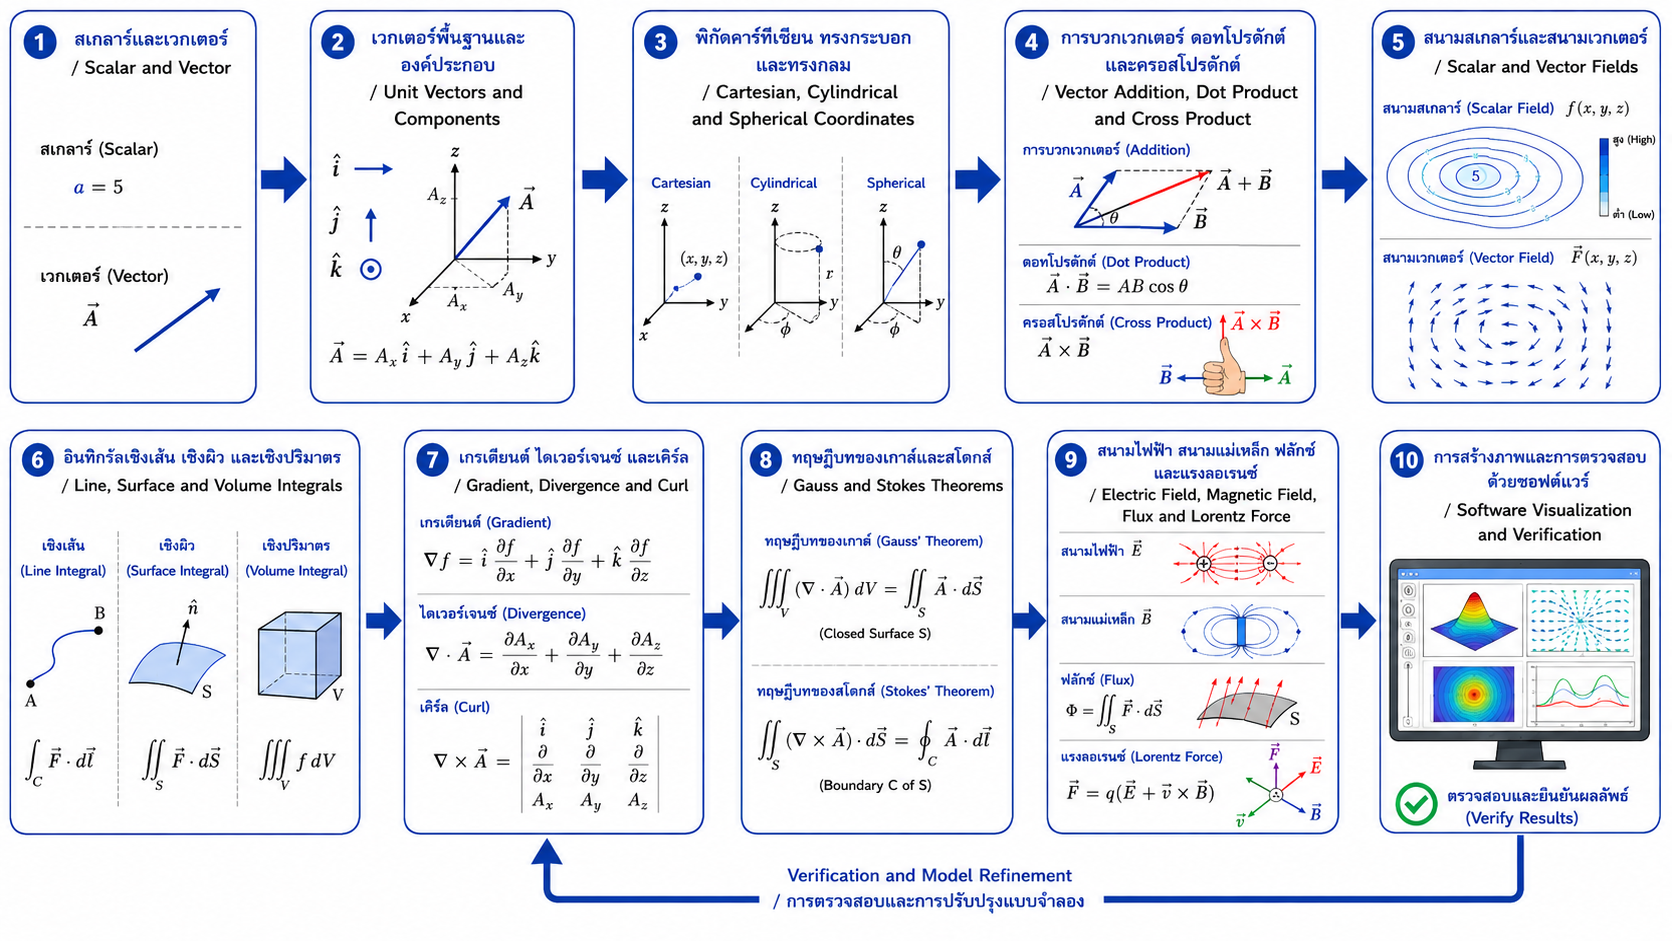
\includegraphics[width=0.8\textwidth]{images/chapter3/figure-01.png}
    \caption{แผนผังการเรียนรู้การวิเคราะห์เวกเตอร์สู่การประยุกต์สนามแม่เหล็กไฟฟ้า}
\end{figure}

\newpage

\subsection{6. บทนำ}

ในวงจรไฟฟ้าแบบรวมศูนย์ เรามักใช้แรงดันและกระแสเป็นค่าที่ขึ้นกับเวลา แต่เมื่อพิจารณาระบบที่มีมิติทางกายภาพ เช่น สายส่ง เสาอากาศ มอเตอร์ไฟฟ้า หม้อแปลง ตัวเก็บประจุ แผ่นนำไฟฟ้า หรือบริเวณรอบตัวนำ ปริมาณทางไฟฟ้าและแม่เหล็กจะแตกต่างกันตามตำแหน่งและทิศทาง การระบุเพียงค่าเดียวจึงไม่เพียงพอ

ตัวอย่างเช่น สนามไฟฟ้ารอบประจุบวกชี้ออกจากประจุในทุกทิศทาง ขณะที่สนามแม่เหล็กรอบลวดตัวนำตรงที่มีกระแสไหลมีทิศเป็นวงกลมล้อมรอบตัวนำ ทิศของแรงบนประจุที่เคลื่อนที่ในสนามแม่เหล็กตั้งฉากกับทั้งทิศความเร็วและทิศสนาม ปรากฏการณ์เหล่านี้ต้องใช้เวกเตอร์และสนามเวกเตอร์ในการอธิบาย

การวิเคราะห์เวกเตอร์ยังช่วยให้กฎทางฟิสิกส์มีรูปแบบกระชับและมีความหมายชัดเจน เช่น

\begin{itemize}
\item \(\mathbf{E}=-\nabla V\) แสดงว่าสนามไฟฟ้าชี้ไปทางที่ศักย์ไฟฟ้าลดลงเร็วที่สุด
\item \(\nabla\cdot\mathbf{D}=\rho_v\) แสดงความสัมพันธ์เฉพาะที่ระหว่างความหนาแน่นฟลักซ์ไฟฟ้ากับความหนาแน่นประจุปริมาตร
\item \(\nabla\cdot\mathbf{B}=0\) สะท้อนว่าเส้นแรงแม่เหล็กไม่มีจุดเริ่มหรือจุดสิ้นสุดแบบประจุแม่เหล็กเดี่ยวในทฤษฎีมาตรฐาน
\item \(\mathbf{F}=q(\mathbf{E}+\mathbf{v}\times\mathbf{B})\) เชื่อมสนามไฟฟ้า สนามแม่เหล็ก และแรงที่กระทำต่อประจุ
\end{itemize}

จุดมุ่งหมายของบทนี้จึงไม่ใช่ให้ผู้เรียนจำสมการจำนวนมาก แต่ให้สามารถมองเห็นโครงสร้างของสนาม เลือกระบบพิกัดให้สอดคล้องกับสมมาตร เลือกผลคูณเวกเตอร์ให้เหมาะกับความหมาย และแปลผลคำนวณกลับไปสู่ปรากฏการณ์ทางวิศวกรรม

\subsection{7. เนื้อหาหลัก การวิเคราะห์เวกเตอร์สำหรับงานวิศวกรรมไฟฟ้า}

\subsubsection{7.1 ความหมายของสเกลาร์และเวกเตอร์}

\paragraph{7.1.1 ปริมาณสเกลาร์}

\textbf{สเกลาร์ (Scalar)} เป็นปริมาณที่กำหนดได้ด้วยขนาดและหน่วย โดยไม่ต้องระบุทิศทาง ตัวอย่างในงานวิศวกรรมไฟฟ้า ได้แก่ ประจุไฟฟ้า ศักย์ไฟฟ้า พลังงาน กำลังไฟฟ้า ความต้านทาน และอุณหภูมิ สเกลาร์อาจเป็นบวก ลบ หรือศูนย์ เครื่องหมายลบไม่ได้หมายถึงทิศทางในอวกาศเสมอไป แต่อาจหมายถึงค่าที่ต่ำกว่าจุดอ้างอิงหรือทิศการถ่ายโอนที่กำหนดตามอนุสัญญา

\paragraph{7.1.2 ปริมาณเวกเตอร์}

\textbf{เวกเตอร์ (Vector)} เป็นปริมาณที่ต้องระบุทั้งขนาดและทิศทาง ตัวอย่าง ได้แก่ ตำแหน่ง \(\mathbf{r}\) ความเร็ว \(\mathbf{v}\) แรง \(\mathbf{F}\) สนามไฟฟ้า \(\mathbf{E}\) ความหนาแน่นฟลักซ์ไฟฟ้า \(\mathbf{D}\) ความเข้มสนามแม่เหล็ก \(\mathbf{H}\) ความหนาแน่นฟลักซ์แม่เหล็ก \(\mathbf{B}\) และความหนาแน่นกระแส \(\mathbf{J}\)

\paragraph{7.1.3 การแทนเวกเตอร์ในพิกัดฉาก}

\[
\mathbf{A}=A_x\mathbf{a}_x+A_y\mathbf{a}_y+A_z\mathbf{a}_z
\]

โดย \(A_x,A_y,A_z\) คือองค์ประกอบตามแกน และ \(\mathbf{a}_x,\mathbf{a}_y,\mathbf{a}_z\) คือเวกเตอร์หนึ่งหน่วย ขนาดของเวกเตอร์คือ

\[
|\mathbf{A}|=\sqrt{A_x^2+A_y^2+A_z^2}
\]

สูตรนี้ใช้เมื่อแกนทั้งสามตั้งฉากกันและเวกเตอร์หนึ่งหน่วยมีขนาดหนึ่ง

% [รูปที่ 2: การแยกเวกเตอร์สามมิติเป็นองค์ประกอบตามแกน]
% ประเภทภาพ: Technical Illustration
% ตำแหน่งที่แนะนำ: หลังหัวข้อ 7.1.3
% วัตถุประสงค์การเรียนรู้: เชื่อมเวกเตอร์เชิงเรขาคณิตกับองค์ประกอบพีชคณิต
% คำอธิบายภาพ: แสดงเวกเตอร์ $\mathbf{A}$ จากจุดกำเนิดไปยังจุด $(A_x,A_y,A_z)$ พร้อมเส้นฉายตั้งฉากและลูกศรองค์ประกอบ
% องค์ประกอบที่ต้องมี: แกน $x,y,z$ จุดกำเนิด เวกเตอร์หลัก เส้นฉายประ และป้ายองค์ประกอบ
% ภาษาของป้ายกำกับ: ไทยและอังกฤษ
% สัดส่วนภาพ: 16:9
% Image Generation Prompt: Clean 3D engineering textbook illustration of a vector A from the origin to point (Ax, Ay, Az) in a Cartesian coordinate system. Show orthogonal projections and component arrows Ax ax, Ay ay and Az az, dashed projection lines, labeled x-y-z axes, white background, precise blue technical line art, 16:9.
% Alt Text: เวกเตอร์สามมิติถูกแยกเป็นองค์ประกอบตามแกนตั้งฉาก $x,y,z$

\begin{figure}[htbp]
    \centering
    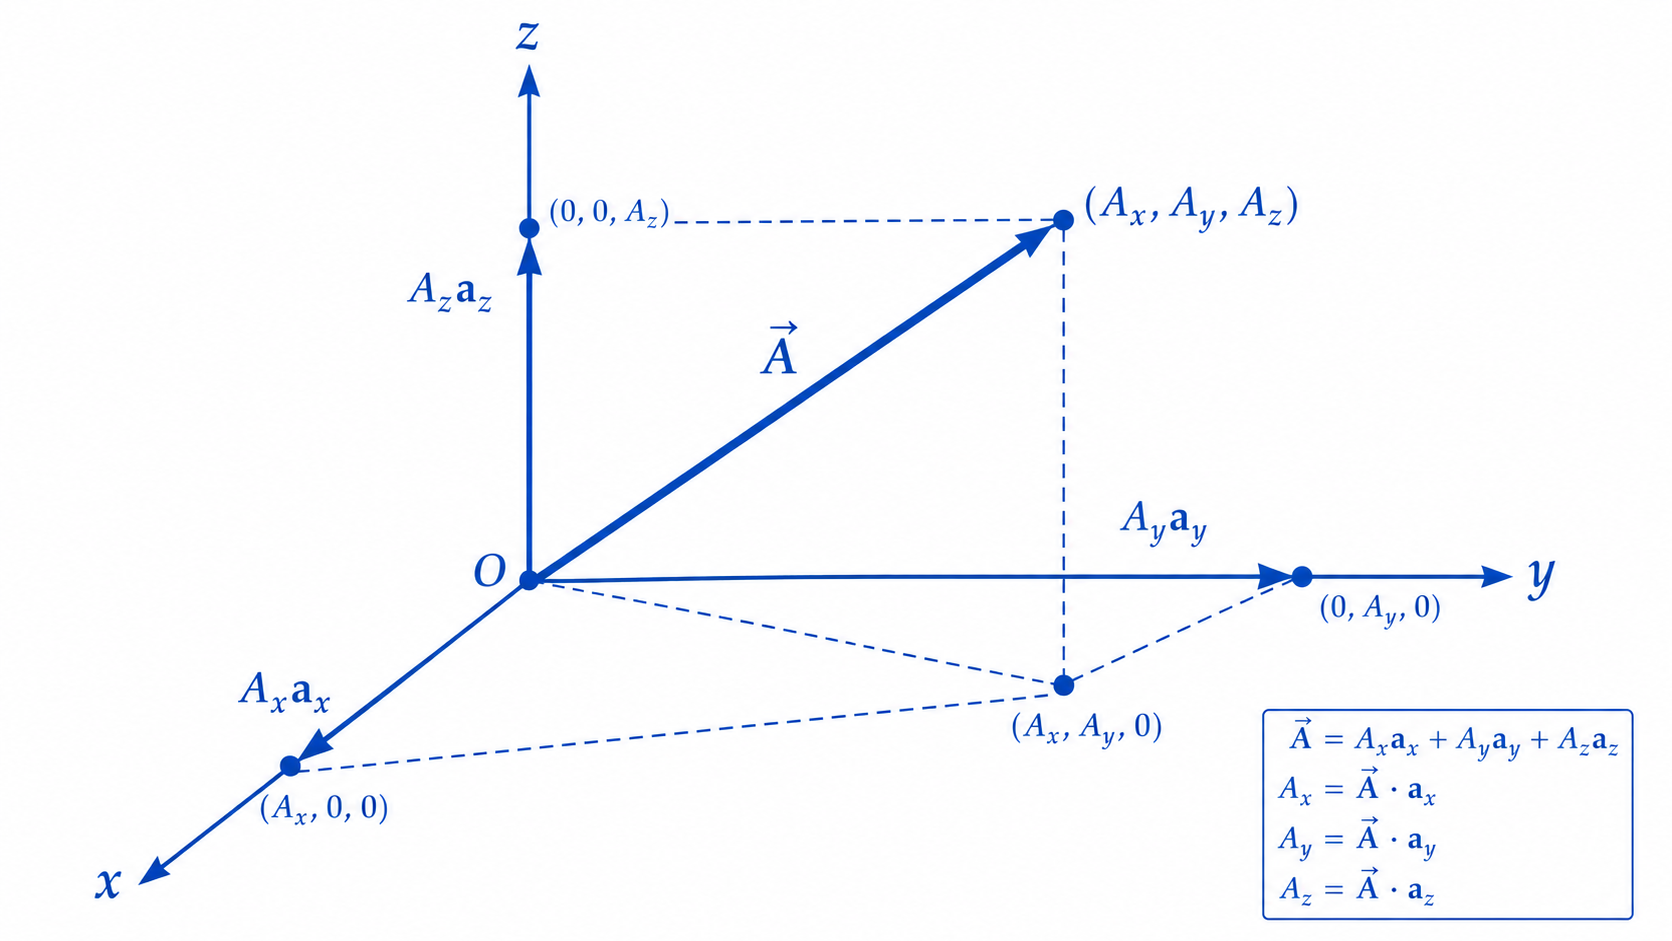
\includegraphics[width=0.8\textwidth]{images/chapter3/figure-02.png}
    \caption{การแยกเวกเตอร์สามมิติเป็นองค์ประกอบตามแกน}
\end{figure}

\paragraph{ตัวอย่างที่ 1 การหาขนาดและเวกเตอร์หนึ่งหน่วย}

กำหนดให้

\[
\mathbf{A}=3\mathbf{a}_x-2\mathbf{a}_y+6\mathbf{a}_z
\]

ขนาดคือ

\[
|\mathbf{A}|=\sqrt{3^2+(-2)^2+6^2}=7
\]

เวกเตอร์หนึ่งหน่วยคือ

\[
\boxed{\mathbf{a}_A=\frac{3}{7}\mathbf{a}_x-\frac{2}{7}\mathbf{a}_y+\frac{6}{7}\mathbf{a}_z}
\]

ตรวจสอบได้ว่า \(|\mathbf{a}_A|=1\) เครื่องหมายลบขององค์ประกอบ \(y\) แสดงว่ามีส่วนชี้ตรงข้ามแกน \(y\) บวก


\subsubsection{7.2 ระบบพิกัดที่ใช้ในงานวิศวกรรมไฟฟ้า}

การเลือกระบบพิกัดที่สอดคล้องกับสมมาตรช่วยลดจำนวนตัวแปรและทำให้สมการง่ายขึ้น

\paragraph{7.2.1 ระบบพิกัดฉาก}

จุดเขียนเป็น \(P(x,y,z)\) และ

\[
\mathbf{r}=x\mathbf{a}_x+y\mathbf{a}_y+z\mathbf{a}_z
\]

\[
d\mathbf{l}=dx\mathbf{a}_x+dy\mathbf{a}_y+dz\mathbf{a}_z,\qquad
dV=dx\,dy\,dz
\]

เหมาะกับแผ่นระนาบ กล่อง และระบบที่เปลี่ยนตามแกนตรง

\paragraph{7.2.2 ระบบพิกัดทรงกระบอก}

จุดเขียนเป็น \(P(\rho,\phi,z)\) โดย

\[
x=\rho\cos\phi,\qquad y=\rho\sin\phi
\]

\[
\rho=\sqrt{x^2+y^2},\qquad \phi=\operatorname{atan2}(y,x)
\]

เวกเตอร์หนึ่งหน่วยสัมพันธ์กับพิกัดฉากดังนี้

\[
\mathbf{a}_\rho=\cos\phi\,\mathbf{a}_x+\sin\phi\,\mathbf{a}_y
\]

\[
\mathbf{a}_\phi=-\sin\phi\,\mathbf{a}_x+\cos\phi\,\mathbf{a}_y
\]

\[
d\mathbf{l}=d\rho\,\mathbf{a}_\rho+\rho d\phi\,\mathbf{a}_\phi+dz\,\mathbf{a}_z
\]

\[
dV=\rho\,d\rho\,d\phi\,dz
\]

เหมาะกับลวดตรง สายโคแอกเชียล และระบบสมมาตรรอบแกน

\paragraph{7.2.3 ระบบพิกัดทรงกลม}

ใช้อนุสัญญา \(P(r,\theta,\phi)\) โดย \(\theta\) วัดลงจากแกน \(z\) บวก และ \(\phi\) วัดในระนาบ \(xy\)

\[
x=r\sin\theta\cos\phi,\quad
y=r\sin\theta\sin\phi,\quad
z=r\cos\theta
\]

\[
d\mathbf{l}=dr\,\mathbf{a}_r+r\,d\theta\,\mathbf{a}_\theta+r\sin\theta\,d\phi\,\mathbf{a}_\phi
\]

\[
dV=r^2\sin\theta\,dr\,d\theta\,d\phi
\]

เหมาะกับประจุจุด ตัวนำทรงกลม และระบบสมมาตรรอบจุด

\begin{quote}
\textbf{ข้อควรระวัง:} ตำราบางเล่มสลับสัญลักษณ์ \(\theta\) กับ \(\phi\) จึงต้องตรวจอนุสัญญาก่อนใช้สูตร
\end{quote}

\paragraph{7.2.4 การเลือกระบบพิกัดจากสมมาตร}

\begin{table}[htbp]
    \centering
    \begin{tabularx}{\textwidth}{L{0.25\textwidth} L{0.27\textwidth} Y}
        \hline
        \textbf{ลักษณะระบบ} & \textbf{ระบบพิกัดที่มักเหมาะสม} & \textbf{ตัวอย่าง} \\
        \hline
        สมมาตรตามระนาบ & พิกัดฉาก & ตัวเก็บประจุแผ่นขนาน \\
        สมมาตรรอบแกน & ทรงกระบอก & ลวดตรง สายโคแอกเชียล \\
        สมมาตรรอบจุด & ทรงกลม & สนามจากประจุจุด \\
        ไม่มีสมมาตรเด่น & พิกัดฉาก/เชิงตัวเลข & อิเล็กโทรดรูปทรงซับซ้อน \\
        \hline
    \end{tabularx}
\end{table}

% [รูปที่ 3: เปรียบเทียบระบบพิกัดฉาก ทรงกระบอก และทรงกลม]
% ประเภทภาพ: Technical Illustration / Infographic
% ตำแหน่งที่แนะนำ: หลังหัวข้อ 7.2.4
% วัตถุประสงค์การเรียนรู้: เห็นนิยามพิกัดและสมมาตรที่เหมาะกับแต่ละระบบ
% คำอธิบายภาพ: สามส่วนแสดงจุดเดียวกันในพิกัดฉาก ทรงกระบอก และทรงกลม พร้อมมุม ระยะ และเวกเตอร์หนึ่งหน่วย
% องค์ประกอบที่ต้องมี: แกนพิกัด เส้นรัศมี ส่วนโค้งมุม และตัวอย่างแผ่นขนาน ลวดตรง ประจุจุด
% ภาษาของป้ายกำกับ: ไทยและอังกฤษ
% สัดส่วนภาพ: 16:9
% Image Generation Prompt: Three-panel engineering textbook comparison of Cartesian, cylindrical and spherical coordinate systems, showing the same point in space with coordinates (x,y,z), (rho,phi,z), and (r,theta,phi). Include axes, projection lines, angle arcs, radial distances, local unit vectors, and small application icons for parallel plates, a long wire, and a point charge. White background, accurate blue technical line art, Thai-English labels, 16:9.
% Alt Text: เปรียบเทียบพิกัดสามระบบและตัวอย่างสมมาตรที่เหมาะสม

\begin{figure}[htbp]
    \centering
    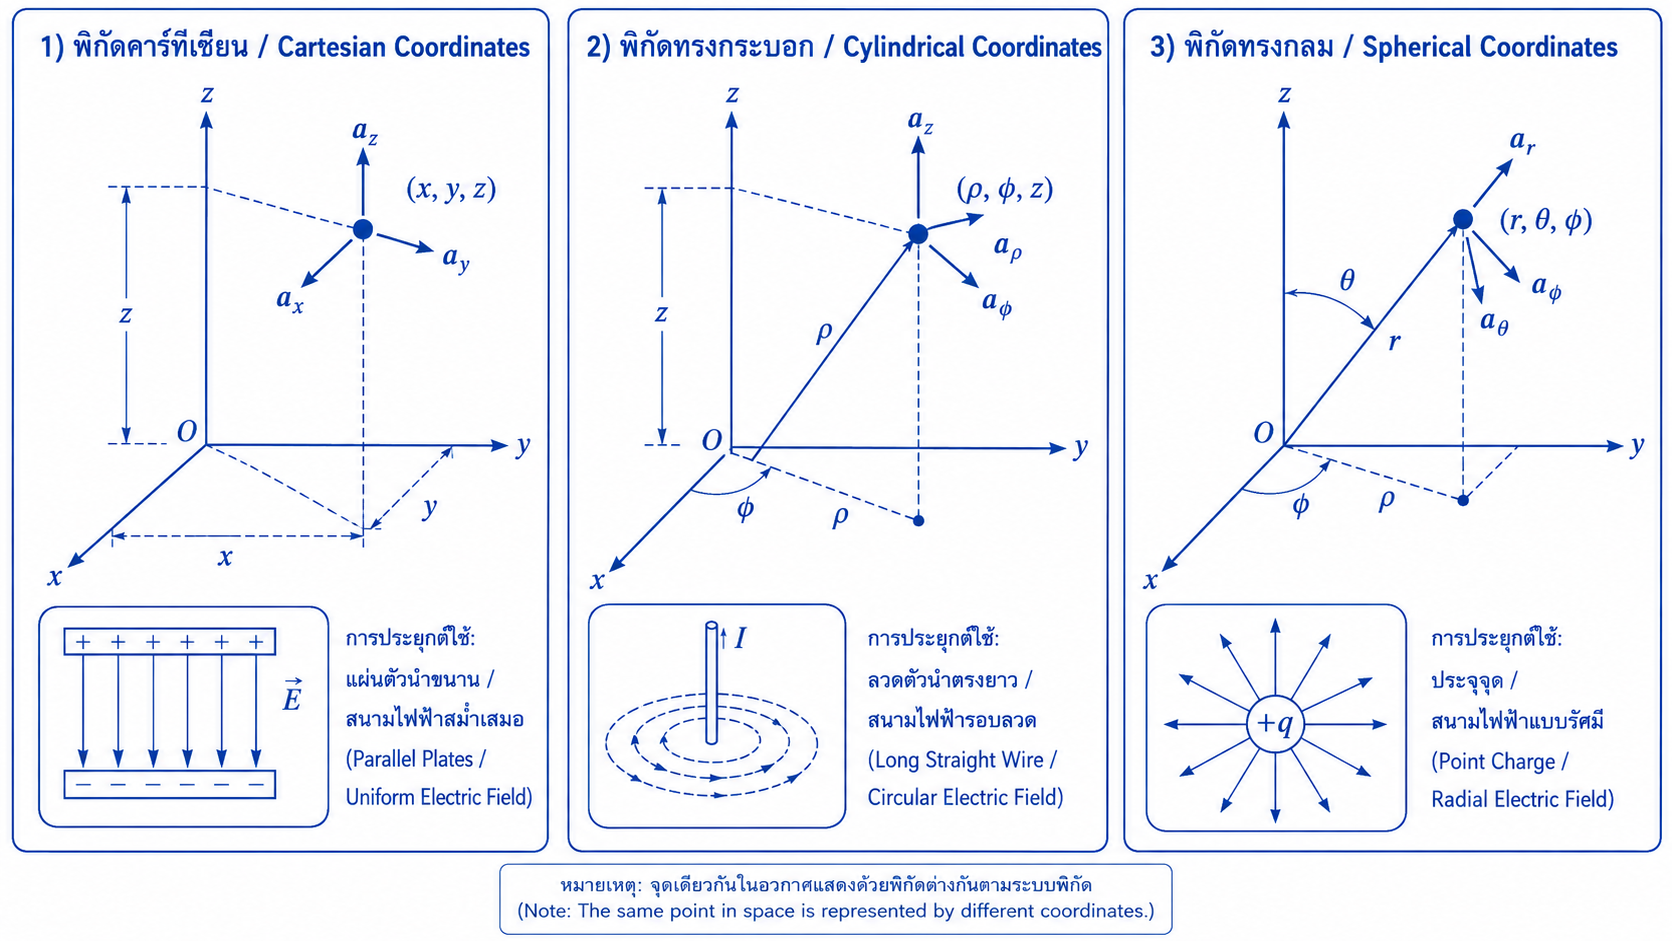
\includegraphics[width=0.8\textwidth]{images/chapter3/figure-03.png}
    \caption{เปรียบเทียบระบบพิกัดฉาก ทรงกระบอก และทรงกลม}
\end{figure}

\paragraph{ตัวอย่างที่ 2 การแปลงพิกัด}

ให้ \(P=(3,4,5)\)

พิกัดทรงกระบอก:

\[
\rho=5,\qquad \phi=\tan^{-1}(4/3)=53.13^\circ
\]

\[
\boxed{P=(5,53.13^\circ,5)}
\]

พิกัดทรงกลม:

\[
r=\sqrt{50}=7.071,\qquad
\theta=\cos^{-1}(5/7.071)=45.00^\circ
\]

\[
\boxed{P=(7.071,45.00^\circ,53.13^\circ)}
\]

\subsubsection{7.3 การบวก ลบ และการคูณเวกเตอร์}

เมื่อเวกเตอร์อยู่ในฐานเดียวกัน

\[
\mathbf{A}\pm\mathbf{B}
=(A_x\pm B_x)\mathbf{a}_x
+(A_y\pm B_y)\mathbf{a}_y
+(A_z\pm B_z)\mathbf{a}_z
\]

การคูณด้วยสเกลาร์ \(k\) ให้ \(k\mathbf{A}\) หาก \(k<0\) ทิศเวกเตอร์กลับตรงข้าม

สำหรับจุด \(P_1(x_1,y_1,z_1)\) และ \(P_2(x_2,y_2,z_2)\)

\[
\mathbf{R}_{12}=(x_2-x_1)\mathbf{a}_x+(y_2-y_1)\mathbf{a}_y+(z_2-z_1)\mathbf{a}_z
\]

\[
R_{12}=|\mathbf{R}_{12}|,\qquad
\mathbf{a}_{12}=\frac{\mathbf{R}_{12}}{R_{12}}
\]

ความสัมพันธ์นี้สำคัญต่อการหาทิศสนามจากแหล่งกำเนิดไปยังจุดสังเกต

\subsubsection{7.4 ดอตโปรดักต์และการประยุกต์กับงานและพลังงาน}

\paragraph{7.4.1 นิยามและความหมาย}

ดอตโปรดักต์หรือผลคูณเชิงสเกลาร์นิยามเป็น

\[
\mathbf{A}\cdot\mathbf{B}=|\mathbf{A}||\mathbf{B}|\cos\theta
\]

โดย \(\theta\) คือมุมระหว่างเวกเตอร์ ผลลัพธ์เป็นสเกลาร์

\begin{itemize}
\item \(\theta=0^\circ\): ผลคูณเป็นบวกสูงสุด
\item \(\theta=90^\circ\): ผลคูณเป็นศูนย์
\item \(90^\circ<\theta\leq180^\circ\): ผลคูณเป็นลบ
\end{itemize}

ในพิกัดฉาก

\[
\mathbf{A}\cdot\mathbf{B}=A_xB_x+A_yB_y+A_zB_z
\]

องค์ประกอบเชิงสเกลาร์ของ \(\mathbf{A}\) ตามทิศเวกเตอร์หนึ่งหน่วย \(\mathbf{a}_u\) คือ

\[
A_u=\mathbf{A}\cdot\mathbf{a}_u
\]

เวกเตอร์ฉายคือ

\[
\operatorname{proj}_{\mathbf{a}_u}\mathbf{A}
=(\mathbf{A}\cdot\mathbf{a}_u)\mathbf{a}_u
\]

\paragraph{7.4.2 งานจากแรงและสนามไฟฟ้า}

งานย่อยจากแรง \(\mathbf{F}\) เมื่อเคลื่อนที่ \(d\mathbf{l}\) คือ

\[
dW=\mathbf{F}\cdot d\mathbf{l}
\]

งานรวมตามเส้นทาง \(C\) คือ

\[
W=\int_C\mathbf{F}\cdot d\mathbf{l}
\]

สำหรับประจุ \(q\) ในสนามไฟฟ้า \(\mathbf{E}\)

\[
W=q\int_C\mathbf{E}\cdot d\mathbf{l}
\]

หน่วยคือ \(\text{N}\cdot\text{m}=\text{J}\) ดอตโปรดักต์เลือกเฉพาะองค์ประกอบของแรงตามทิศการเคลื่อนที่

% [รูปที่ 4: ความหมายเชิงเรขาคณิตของดอตโปรดักต์และครอสโปรดักต์]
% ประเภทภาพ: Infographic / Technical Illustration
% ตำแหน่งที่แนะนำ: หลังหัวข้อ 7.4.2
% วัตถุประสงค์การเรียนรู้: เปรียบเทียบผลคูณที่ให้การฉายกับผลคูณที่ให้เวกเตอร์ตั้งฉาก
% คำอธิบายภาพ: ด้านซ้ายแสดงมุมและเงาฉายของเวกเตอร์ ด้านขวาแสดงพื้นที่สี่เหลี่ยมด้านขนานและเวกเตอร์ปกติตามกฎมือขวา
% องค์ประกอบที่ต้องมี: มุม $\theta$ เส้นฉาย ลูกศรปกติ สูตรดอตและครอส
% ภาษาของป้ายกำกับ: ไทยและอังกฤษ
% สัดส่วนภาพ: 16:9
% Image Generation Prompt: Split-panel engineering textbook illustration comparing dot product and cross product. Left: vectors A and B with angle theta, projection of A onto B, formula A dot B = |A||B|cos theta, scalar result. Right: vectors A and B forming a parallelogram, normal vector A cross B determined by the right-hand rule, formula magnitude = |A||B|sin theta, vector result. White background, clean blue line art, Thai-English labels, 16:9.
% Alt Text: ดอตโปรดักต์แสดงองค์ประกอบตามแนว ส่วนครอสโปรดักต์แสดงเวกเตอร์ตั้งฉาก

\begin{figure}[htbp]
    \centering
    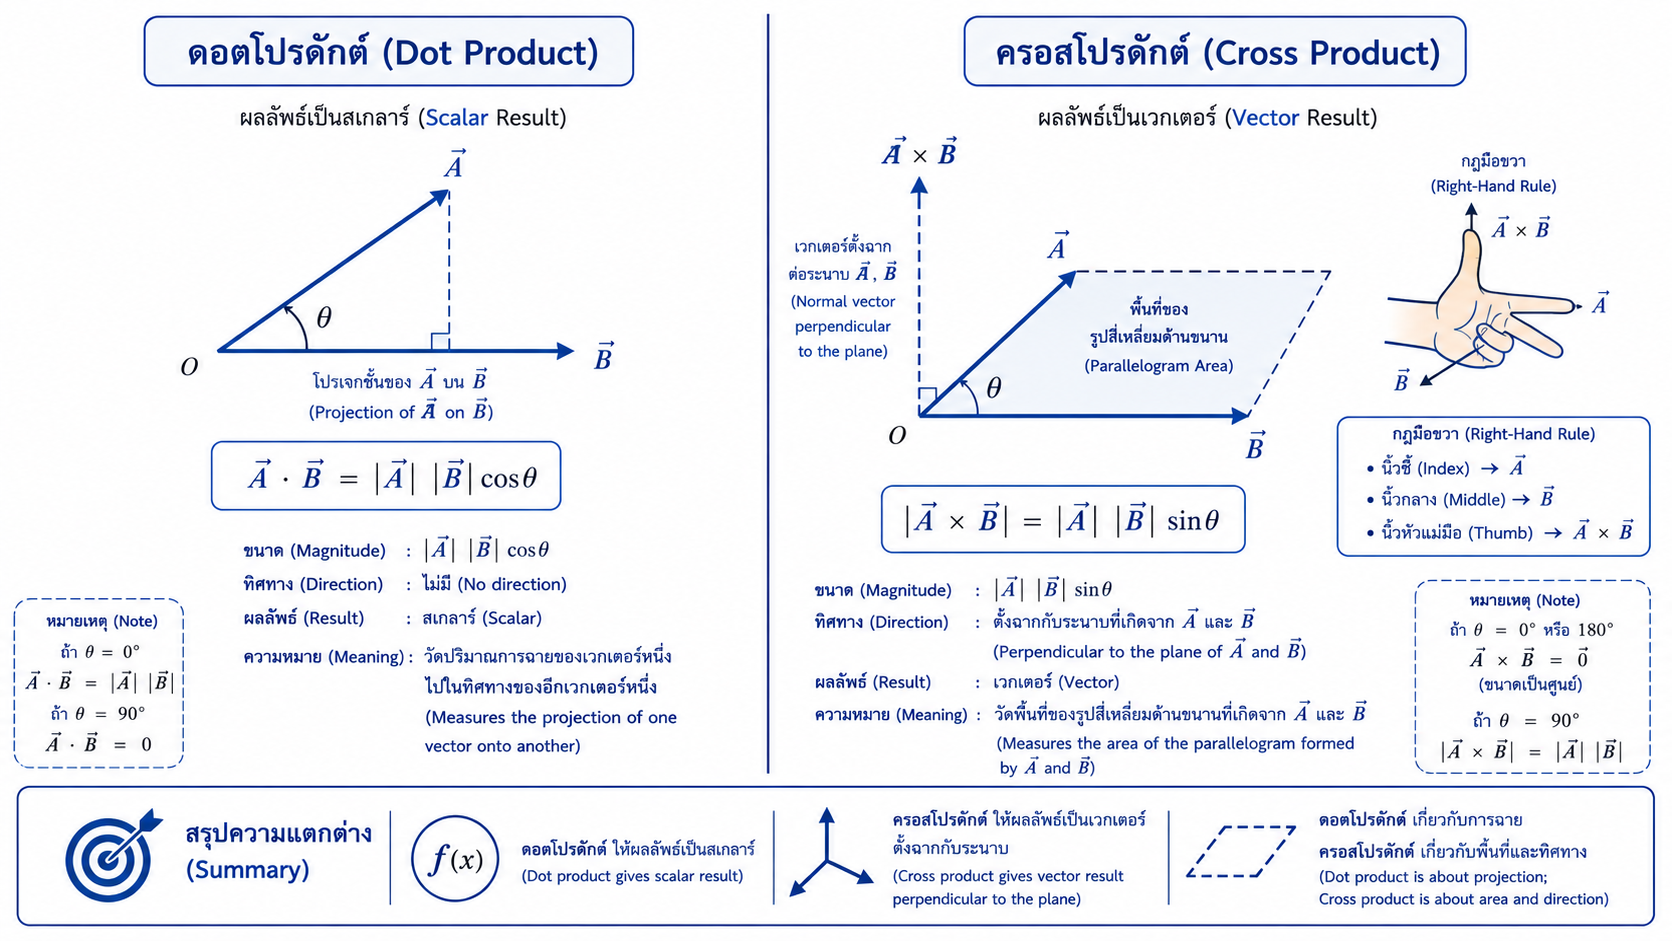
\includegraphics[width=0.8\textwidth]{images/chapter3/figure-04.png}
    \caption{ความหมายเชิงเรขาคณิตของดอตโปรดักต์และครอสโปรดักต์}
\end{figure}

\paragraph{ตัวอย่างที่ 3 ดอตโปรดักต์ มุม และการฉาย}

กำหนด

\[
\mathbf{A}=2\mathbf{a}_x-\mathbf{a}_y+3\mathbf{a}_z,\qquad
\mathbf{B}=\mathbf{a}_x+4\mathbf{a}_y-2\mathbf{a}_z
\]

\begin{enumerate}
\item ดอตโปรดักต์
\end{enumerate}

\[
\mathbf{A}\cdot\mathbf{B}=2-4-6=-8
\]

\begin{enumerate}
\setcounter{enumi}{1}
\item ขนาด
\end{enumerate}

\[
|\mathbf{A}|=\sqrt{14},\qquad |\mathbf{B}|=\sqrt{21}
\]

\begin{enumerate}
\setcounter{enumi}{2}
\item มุม
\end{enumerate}

\[
\cos\theta=\frac{-8}{\sqrt{294}}
\]

\[
\boxed{\theta\approx117.8^\circ}
\]

\begin{enumerate}
\setcounter{enumi}{3}
\item องค์ประกอบของ \(\mathbf{A}\) ตามทิศ \(\mathbf{B}\)
\end{enumerate}

\[
A_B=\frac{\mathbf{A}\cdot\mathbf{B}}{|\mathbf{B}|}
=\frac{-8}{\sqrt{21}}\approx-1.746
\]

ค่าลบแสดงว่าองค์ประกอบที่ฉายชี้สวนทางกับ \(\mathbf{B}\)

\subsubsection{7.5 ครอสโปรดักต์และการประยุกต์กับสนามแม่เหล็ก}

\paragraph{7.5.1 นิยาม}

\[
\mathbf{A}\times\mathbf{B}
=|\mathbf{A}||\mathbf{B}|\sin\theta\,\mathbf{a}_n
\]

\(\mathbf{a}_n\) ตั้งฉากกับระนาบของ \(\mathbf{A}\) และ \(\mathbf{B}\) ตามกฎมือขวา ขนาดของผลคูณเท่ากับพื้นที่สี่เหลี่ยมด้านขนาน

ในพิกัดฉาก

\[
\mathbf{A}\times\mathbf{B}
=
\begin{vmatrix}
\mathbf{a}_x & \mathbf{a}_y & \mathbf{a}_z\\
A_x & A_y & A_z\\
B_x & B_y & B_z
\end{vmatrix}
\]

\[
\mathbf{A}\times\mathbf{B}=-(\mathbf{B}\times\mathbf{A})
\]

\paragraph{7.5.2 แรงแม่เหล็กบนประจุเคลื่อนที่}

\[
\mathbf{F}_m=q\mathbf{v}\times\mathbf{B}
\]

\[
F_m=|q|vB\sin\theta
\]

หาก \(q<0\) ทิศแรงตรงข้ามกับทิศที่กฎมือขวาให้สำหรับประจุบวก

\paragraph{7.5.3 แรงบนตัวนำที่มีกระแส}

สำหรับตัวนำตรงในสนามแม่เหล็กสม่ำเสมอ

\[
\mathbf{F}=I\mathbf{L}\times\mathbf{B}
\]

สมการนี้เป็นพื้นฐานของมอเตอร์ ลำโพง และแอคชูเอเตอร์แม่เหล็กไฟฟ้า

\paragraph{ตัวอย่างที่ 4 แรงบนตัวนำในสนามแม่เหล็ก}

ตัวนำยาว \(0.30\) m วางตาม \(+x\) มีกระแส \(5\) A และอยู่ในสนาม

\[
\mathbf{B}=0.20\mathbf{a}_z\ \text{T}
\]

\[
\mathbf{L}=0.30\mathbf{a}_x\ \text{m}
\]

\[
\mathbf{F}=5(0.30\mathbf{a}_x)\times(0.20\mathbf{a}_z)
\]

เนื่องจาก \(\mathbf{a}_x\times\mathbf{a}_z=-\mathbf{a}_y\)

\[
\boxed{\mathbf{F}=-0.30\mathbf{a}_y\ \text{N}}
\]

ตรวจหน่วยได้ว่า \(\text{A}\cdot\text{m}\cdot\text{T}=\text{N}\)

\subsubsection{7.6 เวกเตอร์หนึ่งหน่วยและองค์ประกอบของเวกเตอร์}

สำหรับเวกเตอร์ไม่เป็นศูนย์

\[
\mathbf{a}_A=\frac{\mathbf{A}}{|\mathbf{A}|}
\]

ถ้า \(\alpha,\beta,\gamma\) เป็นมุมกับแกน \(x,y,z\)

\[
\cos\alpha=\frac{A_x}{|\mathbf{A}|},\quad
\cos\beta=\frac{A_y}{|\mathbf{A}|},\quad
\cos\gamma=\frac{A_z}{|\mathbf{A}|}
\]

\[
\cos^2\alpha+\cos^2\beta+\cos^2\gamma=1
\]

ในพิกัดฉาก เวกเตอร์หนึ่งหน่วยคงทิศทุกตำแหน่ง แต่ในพิกัดทรงกระบอกและทรงกลม ฐานบางตัวเปลี่ยนทิศตามตำแหน่ง เช่น \(\mathbf{a}_\rho\) และ \(\mathbf{a}_\phi\)

การแปลงองค์ประกอบจากฉากเป็นทรงกระบอก:

\[
A_\rho=A_x\cos\phi+A_y\sin\phi
\]

\[
A_\phi=-A_x\sin\phi+A_y\cos\phi,\qquad A_z=A_z
\]

ต้องประเมินที่มุม \(\phi\) ของตำแหน่งนั้น

\subsubsection{7.7 สนามเวกเตอร์ในงานไฟฟ้าและแม่เหล็ก}

\paragraph{7.7.1 สนามสเกลาร์และสนามเวกเตอร์}

สนามสเกลาร์ให้ค่าสเกลาร์ที่ทุกตำแหน่ง เช่น ศักย์ไฟฟ้า

\[
V=V(x,y,z)
\]

พื้นผิวที่ \(V\) คงที่เรียกว่า \textbf{พื้นผิวศักย์เท่ากัน}

สนามเวกเตอร์ให้เวกเตอร์ที่ทุกตำแหน่ง เช่น

\[
\mathbf{E}(x,y,z)=E_x\mathbf{a}_x+E_y\mathbf{a}_y+E_z\mathbf{a}_z
\]

หากขึ้นกับเวลาจะเขียน \(\mathbf{E}(\mathbf{r},t)\)

\paragraph{7.7.2 เส้นสนาม}

เส้นสนามเป็นเส้นสมมติที่เส้นสัมผัสมีทิศเดียวกับสนาม ณ จุดนั้น รูปแบบสำคัญได้แก่

\begin{itemize}
\item สนามสม่ำเสมอ: ลูกศรขนาดและทิศคงที่
\item สนามรัศมี: ชี้ออกหรือเข้าหาศูนย์กลาง
\item สนามวงกลม: ล้อมรอบแกน เช่น สนามแม่เหล็กรอบลวดตรง
\item สนามหมุนวนที่เกิดจากการเปลี่ยนตามเวลา
\end{itemize}

จำนวนเส้นในภาพไม่ใช่ค่าทางกายภาพโดยตรงหากไม่ได้กำหนดสเกล

% [รูปที่ 5: รูปแบบสนามเวกเตอร์ที่พบบ่อย]
% ประเภทภาพ: Infographic / Vector Field Illustration
% ตำแหน่งที่แนะนำ: หลังหัวข้อ 7.7.2
% วัตถุประสงค์การเรียนรู้: จำแนกสนามสม่ำเสมอ สนามรัศมี และสนามวงกลม
% คำอธิบายภาพ: สามช่อง ได้แก่ สนามสม่ำเสมอ สนามไฟฟ้ารัศมีออกจากประจุบวก และสนามแม่เหล็กวงกลมรอบลวดมีกระแส
% องค์ประกอบที่ต้องมี: ลูกศรสนาม ประจุบวก ลวดตรง กระแส $I$ และวงสนาม $\mathbf{B}$
% ภาษาของป้ายกำกับ: ไทยและอังกฤษ
% สัดส่วนภาพ: 16:9
% Image Generation Prompt: Three-panel educational vector field illustration: uniform field with parallel equal arrows; radial electric field pointing outward from a positive point charge with decreasing arrow length versus distance; circular magnetic field around a vertical current-carrying wire with current I upward and right-hand-rule direction. White background, blue engineering textbook style, Thai-English labels, 16:9.
% Alt Text: สนามสม่ำเสมอ สนามไฟฟ้ารัศมี และสนามแม่เหล็กวงกลมรอบลวด

\begin{figure}[htbp]
    \centering
    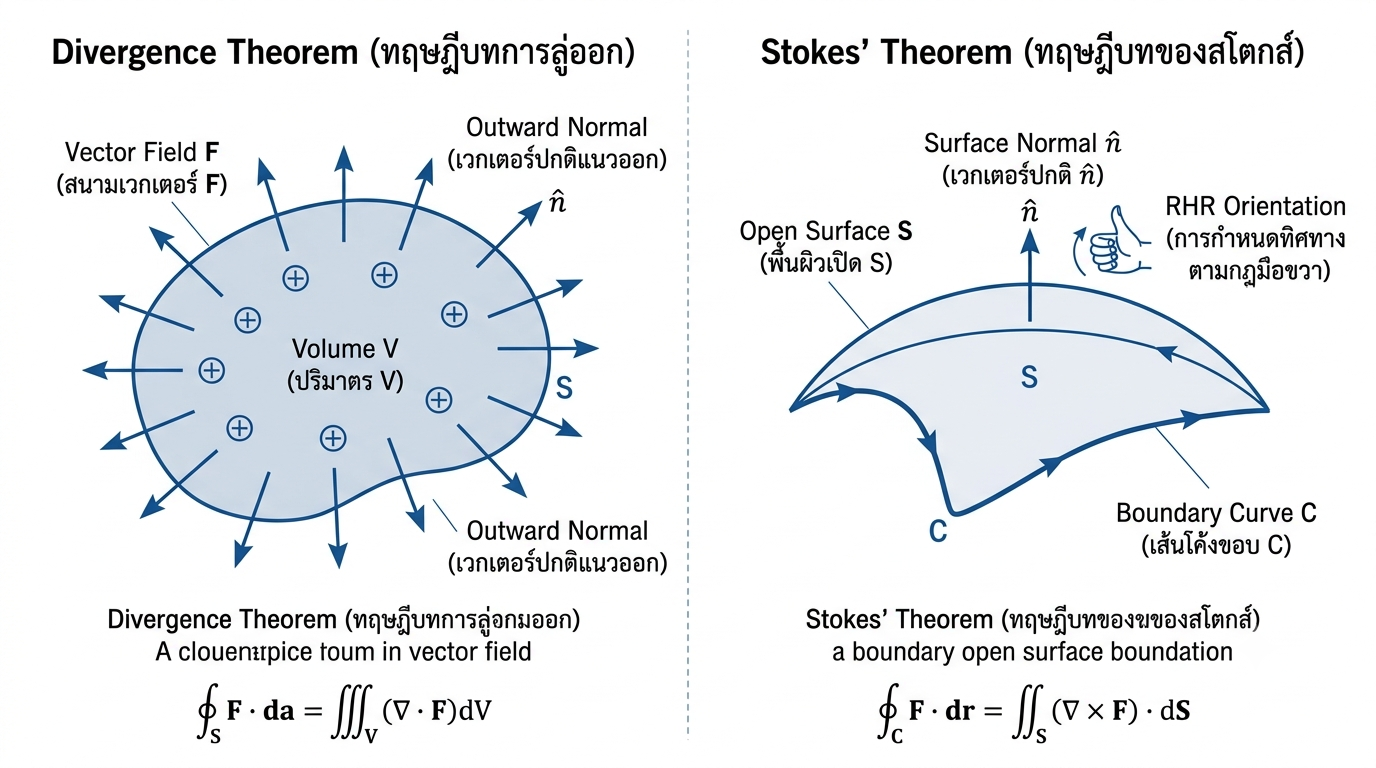
\includegraphics[width=0.8\textwidth]{images/chapter3/figure-05.png}
    \caption{รูปแบบสนามเวกเตอร์ที่พบบ่อย}
\end{figure}

\paragraph{7.7.3 สนามอนุรักษ์และความต่างศักย์}

สนามเรียกว่าอนุรักษ์เมื่ออินทิกรัลระหว่างสองจุดไม่ขึ้นกับเส้นทาง หรือ

\[
\oint_C\mathbf{E}\cdot d\mathbf{l}=0
\]

สำหรับสนามไฟฟ้าสถิต

\[
\mathbf{E}=-\nabla V
\]

\[
V_B-V_A=-\int_A^B\mathbf{E}\cdot d\mathbf{l}
\]

เครื่องหมายลบแสดงว่าสนามไฟฟ้าชี้ไปยังทิศที่ศักย์ลดลง

\subsubsection{7.8 อินทิกรัลเวกเตอร์สำหรับการวิเคราะห์สนาม}

\paragraph{7.8.1 อินทิกรัลเส้น}

\[
\int_C\mathbf{A}\cdot d\mathbf{l}
\]

ใช้คำนวณงาน ความต่างศักย์ และการไหลเวียนตามเส้นทาง

\paragraph{7.8.2 อินทิกรัลพื้นผิวและฟลักซ์}

\[
\Phi=\int_S\mathbf{A}\cdot d\mathbf{S}
\]

โดย \(d\mathbf{S}=\mathbf{a}_n dS\) ดอตโปรดักต์เลือกองค์ประกอบของสนามที่ทะลุผิว

\paragraph{7.8.3 อินทิกรัลปริมาตร}

\[
Q=\int_V\rho_v\,dV
\]

ถ้า \(\rho_v\) มีหน่วย C/m\(^3\) ผลรวม \(Q\) มีหน่วย C

\paragraph{7.8.4 ทิศของขอบเขต}

\begin{itemize}
\item เวกเตอร์ปกติของผิวปิดนิยมชี้ออก
\item ทิศเส้นขอบสัมพันธ์กับเวกเตอร์ปกติด้วยกฎมือขวา
\item การกลับทิศทำให้เครื่องหมายอินทิกรัลเปลี่ยน
\end{itemize}

\paragraph{ตัวอย่างที่ 5 อินทิกรัลเส้นของสนามอนุรักษ์}

ให้

\[
\mathbf{E}=2x\mathbf{a}_x+3y\mathbf{a}_y\ \text{V/m}
\]

จาก \(A=(0,0)\) ไป \(B=(1,2)\) สนามเป็นเกรเดียนต์ของ

\[
\psi=x^2+\frac{3}{2}y^2
\]

ดังนั้น

\[
\int_A^B\mathbf{E}\cdot d\mathbf{l}
=\psi(B)-\psi(A)=1+6=7
\]

\[
\boxed{\int_A^B\mathbf{E}\cdot d\mathbf{l}=7\ \text{V}}
\]

หากใช้ \(V\) เป็นศักย์ไฟฟ้าตาม \(\mathbf{E}=-\nabla V\) จะมีเครื่องหมายตรงข้าม

\subsubsection{7.9 เกรเดียนต์ ไดเวอร์เจนซ์ และเคิร์ล}

\paragraph{7.9.1 ตัวดำเนินการเดล}

ในพิกัดฉาก

\[
\nabla=\mathbf{a}_x\frac{\partial}{\partial x}
+\mathbf{a}_y\frac{\partial}{\partial y}
+\mathbf{a}_z\frac{\partial}{\partial z}
\]

\(\nabla\) เป็นตัวดำเนินการอนุพันธ์ ไม่ใช่เวกเตอร์ทางกายภาพธรรมดา

\paragraph{7.9.2 เกรเดียนต์}

สำหรับสนามสเกลาร์ \(V\)

\[
\nabla V=
\frac{\partial V}{\partial x}\mathbf{a}_x+
\frac{\partial V}{\partial y}\mathbf{a}_y+
\frac{\partial V}{\partial z}\mathbf{a}_z
\]

เกรเดียนต์ชี้ไปยังทิศที่ \(V\) เพิ่มเร็วที่สุด มีขนาดเป็นอัตราการเพิ่มสูงสุดต่อระยะ และตั้งฉากกับพื้นผิว \(V=\text{ค่าคงที่}\)

ในพิกัดทรงกระบอก

\[
\nabla V=
\frac{\partial V}{\partial\rho}\mathbf{a}_\rho+
\frac{1}{\rho}\frac{\partial V}{\partial\phi}\mathbf{a}_\phi+
\frac{\partial V}{\partial z}\mathbf{a}_z
\]

ในพิกัดทรงกลม

\[
\nabla V=
\frac{\partial V}{\partial r}\mathbf{a}_r+
\frac{1}{r}\frac{\partial V}{\partial\theta}\mathbf{a}_\theta+
\frac{1}{r\sin\theta}\frac{\partial V}{\partial\phi}\mathbf{a}_\phi
\]

\paragraph{ตัวอย่างที่ 6 สนามไฟฟ้าจากศักย์}

ให้

\[
V=10-2x^2-y^2-3z\ \text{V}
\]

\[
\nabla V=-4x\mathbf{a}_x-2y\mathbf{a}_y-3\mathbf{a}_z
\]

\[
\mathbf{E}=-\nabla V
=4x\mathbf{a}_x+2y\mathbf{a}_y+3\mathbf{a}_z
\]

ที่ \((1,-2,0)\)

\[
\boxed{\mathbf{E}=4\mathbf{a}_x-4\mathbf{a}_y+3\mathbf{a}_z\ \text{V/m}}
\]

\[
|\mathbf{E}|=\sqrt{41}\approx6.403\ \text{V/m}
\]

\paragraph{7.9.3 ไดเวอร์เจนซ์}

\[
\nabla\cdot\mathbf{A}
=\frac{\partial A_x}{\partial x}
+\frac{\partial A_y}{\partial y}
+\frac{\partial A_z}{\partial z}
\]

ผลเป็นสเกลาร์และบอกฟลักซ์แผ่ออกสุทธิต่อหน่วยปริมาตร

\begin{itemize}
\item บวก: แหล่งกำเนิดสุทธิ
\item ลบ: แหล่งดูดสุทธิ
\item ศูนย์: ไม่มีการไหลออกสุทธิ ณ จุดนั้น แต่สนามอาจไม่เป็นศูนย์
\end{itemize}

ในพิกัดทรงกระบอก

\[
\nabla\cdot\mathbf{A}
=\frac{1}{\rho}\frac{\partial(\rho A_\rho)}{\partial\rho}
+\frac{1}{\rho}\frac{\partial A_\phi}{\partial\phi}
+\frac{\partial A_z}{\partial z}
\]

ในพิกัดทรงกลม

\[
\nabla\cdot\mathbf{A}
=\frac{1}{r^2}\frac{\partial(r^2A_r)}{\partial r}
+\frac{1}{r\sin\theta}\frac{\partial(\sin\theta A_\theta)}{\partial\theta}
+\frac{1}{r\sin\theta}\frac{\partial A_\phi}{\partial\phi}
\]

\paragraph{ตัวอย่างที่ 7 การหาไดเวอร์เจนซ์}

\[
\mathbf{A}=x^2\mathbf{a}_x+xy\mathbf{a}_y+z^2\mathbf{a}_z
\]

\[
\nabla\cdot\mathbf{A}=2x+x+2z=3x+2z
\]

ที่ \((1,2,3)\)

\[
\boxed{\nabla\cdot\mathbf{A}=9}
\]

\paragraph{7.9.4 เคิร์ล}

ในพิกัดฉาก

\[
\nabla\times\mathbf{A}
=
\begin{vmatrix}
\mathbf{a}_x & \mathbf{a}_y & \mathbf{a}_z\\
\dfrac{\partial}{\partial x} & \dfrac{\partial}{\partial y} & \dfrac{\partial}{\partial z}\\
A_x & A_y & A_z
\end{vmatrix}
\]

หรือ

\[
\nabla\times\mathbf{A}
=\left(\frac{\partial A_z}{\partial y}-\frac{\partial A_y}{\partial z}\right)\mathbf{a}_x
+\left(\frac{\partial A_x}{\partial z}-\frac{\partial A_z}{\partial x}\right)\mathbf{a}_y
+\left(\frac{\partial A_y}{\partial x}-\frac{\partial A_x}{\partial y}\right)\mathbf{a}_z
\]

ผลเป็นเวกเตอร์บอกแกนและความเข้มของแนวโน้มการหมุนวนเฉพาะที่

ในพิกัดทรงกระบอก

\[
\begin{aligned}
\nabla\times\mathbf{A}
={}&\frac{1}{\rho}\left[\frac{\partial A_z}{\partial\phi}
-\frac{\partial(\rho A_\phi)}{\partial z}\right]\mathbf{a}_\rho\\
&+\left[\frac{\partial A_\rho}{\partial z}
-\frac{\partial A_z}{\partial\rho}\right]\mathbf{a}_\phi\\
&+\frac{1}{\rho}\left[\frac{\partial(\rho A_\phi)}{\partial\rho}
-\frac{\partial A_\rho}{\partial\phi}\right]\mathbf{a}_z
\end{aligned}
\]

ในพิกัดทรงกลม

\[
\begin{aligned}
\nabla\times\mathbf{A}
={}&\frac{1}{r\sin\theta}
\left[\frac{\partial(\sin\theta A_\phi)}{\partial\theta}
-\frac{\partial A_\theta}{\partial\phi}\right]\mathbf{a}_r\\
&+\frac{1}{r}
\left[\frac{1}{\sin\theta}\frac{\partial A_r}{\partial\phi}
-\frac{\partial(rA_\phi)}{\partial r}\right]\mathbf{a}_\theta\\
&+\frac{1}{r}
\left[\frac{\partial(rA_\theta)}{\partial r}
-\frac{\partial A_r}{\partial\theta}\right]\mathbf{a}_\phi
\end{aligned}
\]

\paragraph{ตัวอย่างที่ 8 สนามหมุน}

\[
\mathbf{A}=-y\mathbf{a}_x+x\mathbf{a}_y
\]

\[
\nabla\times\mathbf{A}
=\left(\frac{\partial x}{\partial x}
-\frac{\partial(-y)}{\partial y}\right)\mathbf{a}_z
=2\mathbf{a}_z
\]

\[
\boxed{\nabla\times\mathbf{A}=2\mathbf{a}_z}
\]

สนามหมุนทวนเข็มนาฬิกาเมื่อมองจาก \(+z\)

\paragraph{7.9.5 เอกลักษณ์เวกเตอร์สำคัญ}

เมื่อฟังก์ชันเรียบเพียงพอ

\[
\nabla\times(\nabla V)=\mathbf{0}
\]

\[
\nabla\cdot(\nabla\times\mathbf{A})=0
\]

\[
\nabla^2V=\nabla\cdot(\nabla V)
\]

\(\nabla^2V\) เรียกว่า \textbf{ลาปลาเซียน} และเป็นพื้นฐานของสมการลาปลาซและปัวซอง

% [รูปที่ 6: ความหมายเชิงภาพของเกรเดียนต์ ไดเวอร์เจนซ์ และเคิร์ล]
% ประเภทภาพ: Infographic
% ตำแหน่งที่แนะนำ: หลังหัวข้อ 7.9.5
% วัตถุประสงค์การเรียนรู้: แยกความหมายของตัวดำเนินการทั้งสาม
% คำอธิบายภาพ: เกรเดียนต์บนเส้นชั้นค่า ไดเวอร์เจนซ์แบบแหล่งกำเนิด/แหล่งดูด และเคิร์ลพร้อมใบพัดเล็ก
% องค์ประกอบที่ต้องมี: เส้นชั้นค่า ลูกศร $\nabla V$ กล่องฟลักซ์เข้า–ออก และแกนหมุน
% ภาษาของป้ายกำกับ: ไทยและอังกฤษ
% สัดส่วนภาพ: 16:9
% Image Generation Prompt: Three-panel educational engineering infographic explaining gradient, divergence and curl. Gradient panel: scalar contour map with gradient arrow normal to contours toward maximum increase. Divergence panel: small control volumes showing source, sink and zero-net-flow cases. Curl panel: circulating vector field with a tiny paddle wheel and rotation axis following the right-hand rule. White background, blue technical textbook style, Thai-English labels, 16:9.
% Alt Text: เกรเดียนต์เป็นทิศเพิ่มสูงสุด ไดเวอร์เจนซ์เป็นการไหลออกสุทธิ และเคิร์ลเป็นการหมุนวนเฉพาะที่

\begin{figure}[htbp]
    \centering
    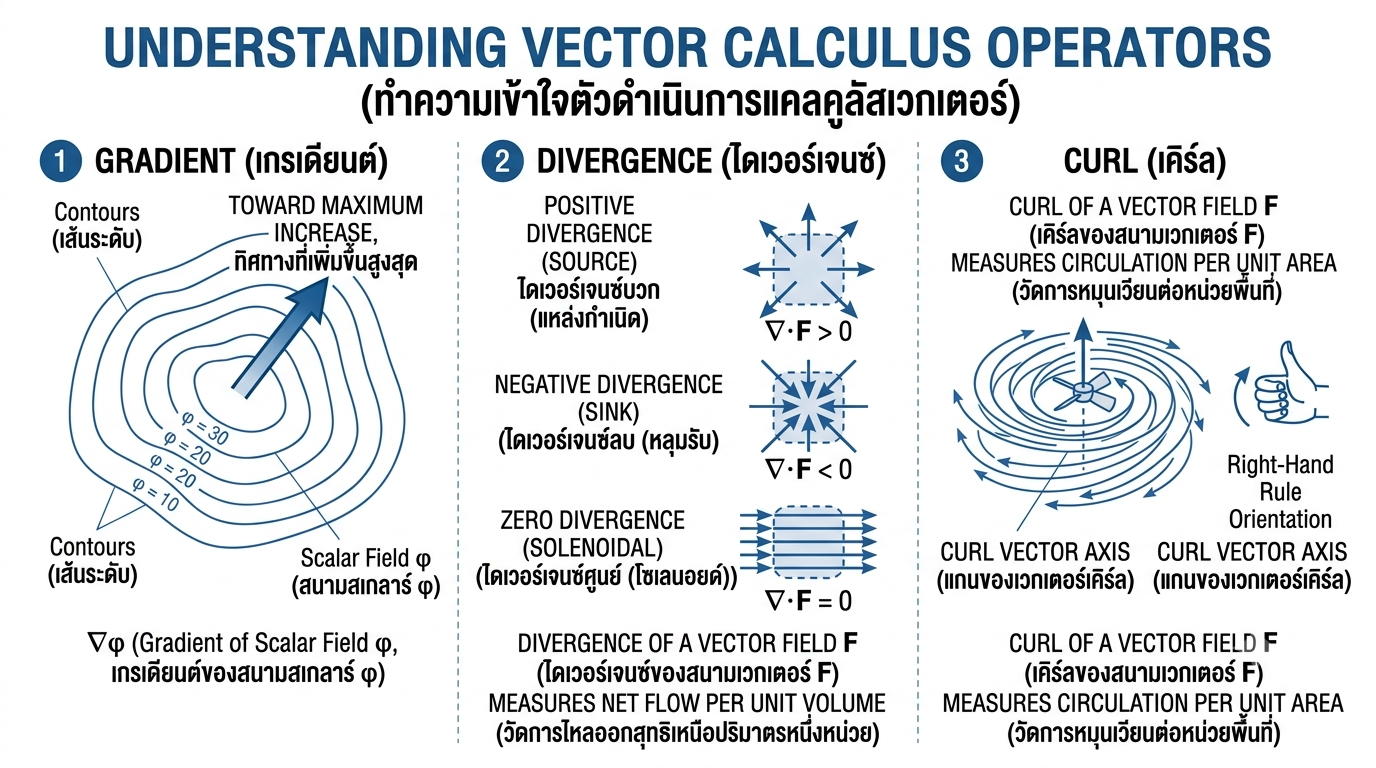
\includegraphics[width=0.8\textwidth]{images/chapter3/figure-06.png}
    \caption{ความหมายเชิงภาพของเกรเดียนต์ ไดเวอร์เจนซ์ และเคิร์ล}
\end{figure}

\paragraph{7.9.6 ตารางสรุป}

\begin{table}[htbp]
    \centering
    \begin{tabularx}{\textwidth}{L{0.18\textwidth} L{0.12\textwidth} L{0.14\textwidth} L{0.22\textwidth} Y}
        \hline
        \textbf{ตัวดำเนินการ} & \textbf{อินพุต} & \textbf{เอาต์พุต} & \textbf{ความหมาย} & \textbf{ตัวอย่างทางไฟฟ้า} \\
        \hline
        \(\nabla V\) & สเกลาร์ & เวกเตอร์ & ทิศเพิ่มเร็วที่สุด & \(\mathbf{E}=-\nabla V\) \\
        \(\nabla\cdot\mathbf{A}\) & เวกเตอร์ & สเกลาร์ & ฟลักซ์ออกสุทธิ & \(\nabla\cdot\mathbf{D}=\rho_v\) \\
        \(\nabla\times\mathbf{A}\) & เวกเตอร์ & เวกเตอร์ & การหมุนวนเฉพาะที่ & กฎฟาราเดย์/แอมแปร์--แมกซ์เวลล์ \\
        \(\nabla^2V\) & สเกลาร์ & สเกลาร์ & ความโค้งสุทธิ & สมการลาปลาซ/ปัวซอง \\
        \hline
    \end{tabularx}
\end{table}

\subsubsection{7.10 ทฤษฎีบทอินทิกรัลของสนาม}

\paragraph{7.10.1 ทฤษฎีบทไดเวอร์เจนซ์}

\[
\oint_S\mathbf{A}\cdot d\mathbf{S}
=\int_V(\nabla\cdot\mathbf{A})\,dV
\]

ฟลักซ์สุทธิที่ออกจากผิวปิดเท่ากับผลรวมความเป็นแหล่งกำเนิดในปริมาตร สนามและอนุพันธ์ต้องเรียบพอ หากมีจุดเอกฐานต้องจัดการอย่างระมัดระวัง

\paragraph{7.10.2 ทฤษฎีบทของสโตกส์}

\[
\oint_C\mathbf{A}\cdot d\mathbf{l}
=\int_S(\nabla\times\mathbf{A})\cdot d\mathbf{S}
\]

ทิศของ \(C\) ต้องสัมพันธ์กับเวกเตอร์ปกติของ \(S\) ตามกฎมือขวา การไหลเวียนรอบเส้นปิดเท่ากับฟลักซ์ของเคิร์ลผ่านพื้นผิว

% [รูปที่ 7: ความเชื่อมโยงรูปอินทิกรัลและรูปอนุพันธ์ของสนาม]
% ประเภทภาพ: Technical Illustration
% ตำแหน่งที่แนะนำ: หลังหัวข้อ 7.10.2
% วัตถุประสงค์การเรียนรู้: เชื่อมฟลักซ์กับไดเวอร์เจนซ์ และการไหลเวียนกับเคิร์ล
% คำอธิบายภาพ: ด้านซ้ายเป็นผิวปิดและแหล่งกำเนิดภายใน ด้านขวาเป็นพื้นผิวเปิด ขอบ $C$ และเวกเตอร์ปกติ
% องค์ประกอบที่ต้องมี: ผิว $S$ ปริมาตร $V$ เส้นขอบ $C$ เวกเตอร์ปกติ และกฎมือขวา
% ภาษาของป้ายกำกับ: ไทยและอังกฤษ
% สัดส่วนภาพ: 16:9
% Image Generation Prompt: Split engineering textbook diagram. Left: a closed surface S enclosing volume V, vector field arrows crossing outward and source symbols inside, labeled Divergence Theorem. Right: an open surface S bounded by curve C, circulation arrows around C, surface normal and right-hand-rule orientation, labeled Stokes' Theorem. White background, accurate blue technical line art, Thai-English labels, 16:9.
% Alt Text: ฟลักซ์ผ่านผิวปิดสัมพันธ์กับไดเวอร์เจนซ์ และการไหลเวียนสัมพันธ์กับเคิร์ล

\begin{figure}[htbp]
    \centering
    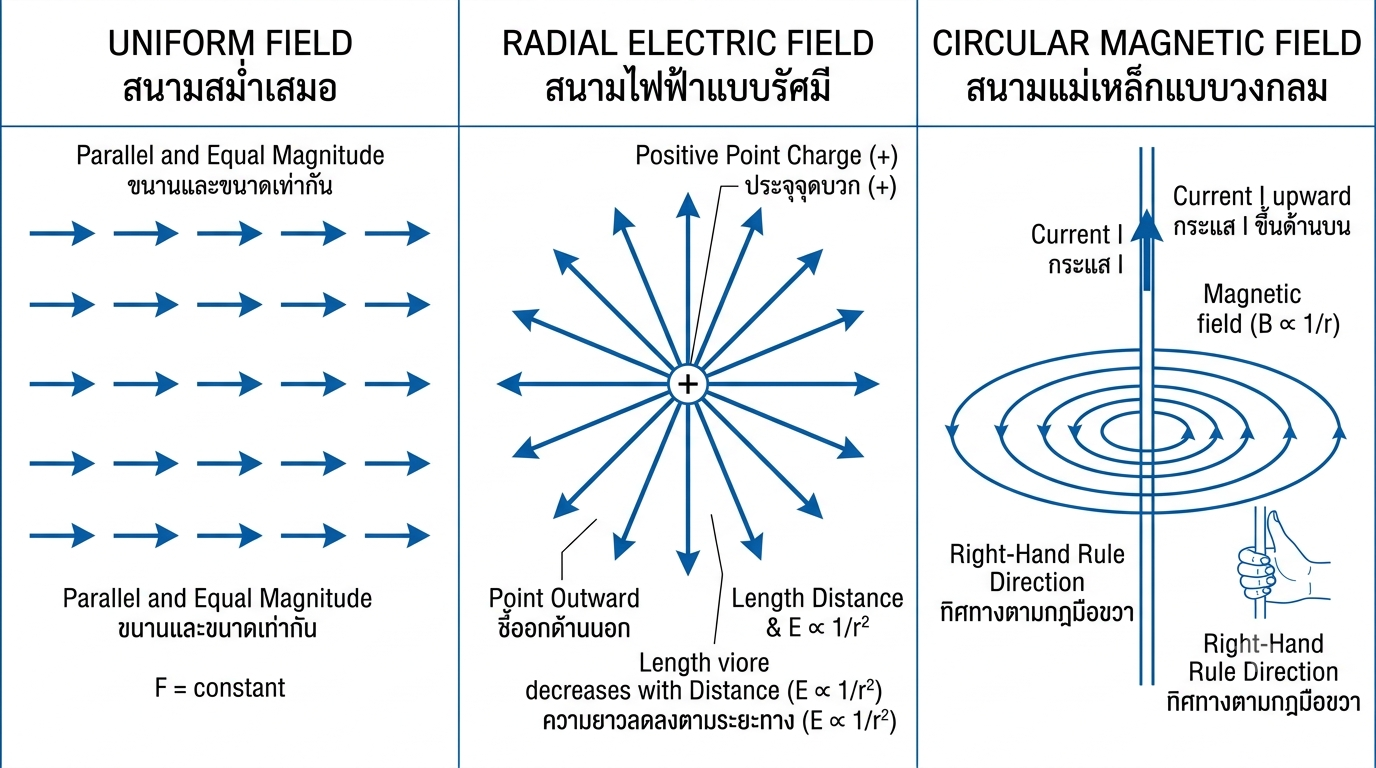
\includegraphics[width=0.8\textwidth]{images/chapter3/figure-07.png}
    \caption{ความเชื่อมโยงรูปอินทิกรัลและรูปอนุพันธ์ของสนาม}
\end{figure}

\subsubsection{7.11 แนวคิดเบื้องต้นของทฤษฎีสนามแม่เหล็กไฟฟ้า}

\paragraph{7.11.1 สนามไฟฟ้าจากประจุจุด}

ในสุญญากาศ สนามไฟฟ้าจากประจุจุด \(Q\) ที่จุดกำเนิดคือ

\[
\mathbf{E}=\frac{Q}{4\pi\varepsilon_0r^2}\mathbf{a}_r
\]

โดย \(Q\) หน่วย C, \(r\) หน่วย m, \(\varepsilon_0\approx8.854\times10^{-12}\) F/m และ \(\mathbf{a}_r\) ชี้ออกจากต้นกำเนิด หาก \(Q<0\) สนามชี้เข้า

\paragraph{7.11.2 หลักการซ้อนทับ}

สำหรับประจุหลายตัว

\[
\mathbf{E}_{\text{total}}=\sum_{i=1}^{N}\mathbf{E}_i
\]

หลักการซ้อนทับใช้เมื่อความสัมพันธ์ของระบบเป็นเชิงเส้นในช่วงที่พิจารณา

\paragraph{7.11.3 กฎของเกาส์}

รูปอินทิกรัล:

\[
\oint_S\mathbf{D}\cdot d\mathbf{S}=Q_{\text{enclosed}}
\]

รูปอนุพันธ์:

\[
\nabla\cdot\mathbf{D}=\rho_v
\]

กฎของเกาส์มีประสิทธิภาพสูงเมื่อมีสมมาตรทรงกลม ทรงกระบอก หรือระนาบชัดเจน ไม่ใช่เพียงเพราะเลือกผิวปิดใด ๆ แล้วจะคำนวณสนามได้ง่ายเสมอ

\paragraph{7.11.4 สนามแม่เหล็กรอบลวดตรงยาว}

สำหรับลวดตรงยาวมาก

\[
\mathbf{B}=\frac{\mu_0I}{2\pi\rho}\mathbf{a}_\phi
\]

โดย \(\mu_0=4\pi\times10^{-7}\) H/m และ \(\rho\) คือระยะตั้งฉากจากลวด ทิศ \(\mathbf{a}_\phi\) เป็นวงกลมรอบลวดตามกฎมือขวา

\paragraph{7.11.5 กฎของแอมแปร์ในกรณีสถิต}

\[
\oint_C\mathbf{H}\cdot d\mathbf{l}=I_{\text{enclosed}}
\]

ใช้ได้สะดวกเมื่อสมมาตรทำให้ \(\mathbf{H}\) สัมผัสเส้นทางและมีขนาดคงที่ตามส่วนสำคัญของเส้นทาง เช่น วงกลมรอบลวดตรงยาว

\paragraph{7.11.6 สมการแมกซ์เวลล์ในภาพรวม}

\begin{table}[htbp]
    \centering
    \begin{tabularx}{\textwidth}{L{0.20\textwidth} L{0.28\textwidth} Y}
        \hline
        \textbf{กฎ} & \textbf{รูปอนุพันธ์} & \textbf{ความหมายเชิงแนวคิด} \\
        \hline
        เกาส์สำหรับไฟฟ้า & \(\nabla\cdot\mathbf{D}=\rho_v\) & ประจุเป็นแหล่งของฟลักซ์ไฟฟ้า \\
        เกาส์สำหรับแม่เหล็ก & \(\nabla\cdot\mathbf{B}=0\) & ฟลักซ์แม่เหล็กผ่านผิวปิดสุทธิเป็นศูนย์ \\
        ฟาราเดย์ & \(\nabla\times\mathbf{E}=-\dfrac{\partial\mathbf{B}}{\partial t}\) & สนามแม่เหล็กที่เปลี่ยนตามเวลาสร้างสนามไฟฟ้าหมุนวน \\
        แอมแปร์--แมกซ์เวลล์ & \(\nabla\times\mathbf{H}=\mathbf{J}+\dfrac{\partial\mathbf{D}}{\partial t}\) & กระแสและสนามไฟฟ้าที่เปลี่ยนตามเวลาสร้างสนามแม่เหล็กหมุนวน \\
        \hline
    \end{tabularx}
\end{table}

บทนี้มุ่งอ่านความหมายของสมการผ่านแนวคิด grad--div--curl ยังไม่มุ่งแก้ปัญหาสนามแม่เหล็กไฟฟ้าเต็มรูปแบบ

\subsubsection{7.12 การประยุกต์เวกเตอร์กับสนามไฟฟ้า สนามแม่เหล็ก และแรง}

\paragraph{7.12.1 สนามไฟฟ้าจากประจุจุด}

ประจุ \(Q=5\) nC อยู่ที่จุดกำเนิด จงหาสนามที่ \(r=0.20\) m

\[
E=\frac{1}{4\pi\varepsilon_0}\frac{Q}{r^2}
\]

\[
E=(8.987\times10^9)\frac{5\times10^{-9}}{(0.20)^2}
\approx1.123\times10^3\ \text{V/m}
\]

\[
\boxed{\mathbf{E}\approx1.123\times10^3\mathbf{a}_r\ \text{V/m}}
\]

สนามชี้ออกเพราะประจุเป็นบวก และลดลงตาม \(1/r^2\)

\paragraph{7.12.2 แรงไฟฟ้าบนประจุ}

ถ้า \(q=2\ \mu\text{C}\) อยู่ในสนาม

\[
\mathbf{E}=(3\mathbf{a}_x-4\mathbf{a}_y)\ \text{kV/m}
\]

\[
\mathbf{F}=q\mathbf{E}
\]

\[
\boxed{\mathbf{F}=6\mathbf{a}_x-8\mathbf{a}_y\ \text{mN}}
\]

\[
|\mathbf{F}|=10\ \text{mN}
\]

\paragraph{7.12.3 แรงลอเรนซ์รวม}

\[
\mathbf{F}=q(\mathbf{E}+\mathbf{v}\times\mathbf{B})
\]

ส่วนไฟฟ้าสามารถทำงานและเปลี่ยนพลังงานจลน์ ส่วนแม่เหล็กตั้งฉากกับความเร็ว ณ ขณะนั้น จึงเปลี่ยนทิศแต่ไม่เปลี่ยนพลังงานจลน์ในกรณีสนามแม่เหล็กเพียงอย่างเดียว

\paragraph{ตัวอย่างที่ 9 แรงแม่เหล็กบนอิเล็กตรอน}

\[
\mathbf{v}=2.0\times10^6\mathbf{a}_x\ \text{m/s},\qquad
\mathbf{B}=0.20\mathbf{a}_z\ \text{T}
\]

สำหรับอิเล็กตรอน \(q=-1.602\times10^{-19}\) C

\[
\mathbf{v}\times\mathbf{B}
=-4.0\times10^5\mathbf{a}_y
\]

\[
\boxed{\mathbf{F}_m=6.408\times10^{-14}\mathbf{a}_y\ \text{N}}
\]

กฎมือขวาให้ทิศ \(\mathbf{v}\times\mathbf{B}\) สำหรับประจุบวก จึงต้องกลับทิศเมื่อเป็นอิเล็กตรอน

\paragraph{7.12.4 สนามแม่เหล็กรอบลวดตรง}

ลวดตรงมีกระแส \(I=10\) A ที่ระยะ \(\rho=0.05\) m

\[
B=\frac{\mu_0I}{2\pi\rho}
=4.0\times10^{-5}\ \text{T}
\]

\[
\boxed{\mathbf{B}=40\ \mu\text{T}\,\mathbf{a}_\phi}
\]

% [รูปที่ 8: ทิศแรงไฟฟ้าและแรงแม่เหล็กบนประจุและตัวนำ]
% ประเภทภาพ: Technical Illustration
% ตำแหน่งที่แนะนำ: หลังหัวข้อ 7.12.4
% วัตถุประสงค์การเรียนรู้: ฝึกอ่านทิศของ $q\mathbf{E}$, $q\mathbf{v}\times\mathbf{B}$ และ $I\mathbf{L}\times\mathbf{B}$
% คำอธิบายภาพ: สามส่วนแสดงประจุบวก/ลบในสนามไฟฟ้า ประจุเคลื่อนที่ในสนามแม่เหล็ก และตัวนำมีกระแสในสนามแม่เหล็ก
% องค์ประกอบที่ต้องมี: ลูกศร $\mathbf{E},\mathbf{v},\mathbf{B},\mathbf{F}$ กระแส $I$ และสัญลักษณ์จุด/กากบาท
% ภาษาของป้ายกำกับ: ไทยและอังกฤษ
% สัดส่วนภาพ: 16:9
% Image Generation Prompt: Three-panel engineering textbook illustration of force directions. Panel 1: positive and negative charges in a uniform electric field E, showing F=qE. Panel 2: moving charge with velocity v in magnetic field B, showing v cross B by right-hand rule and reversed force for a negative charge. Panel 3: current-carrying conductor with vector L in magnetic field B, showing F=I L cross B. Include x-y-z axes and dot/cross symbols. White background, blue technical style, Thai-English labels, 16:9.
% Alt Text: ทิศแรงไฟฟ้าและแรงแม่เหล็กด้วยกฎมือขวา

\begin{figure}[htbp]
    \centering
    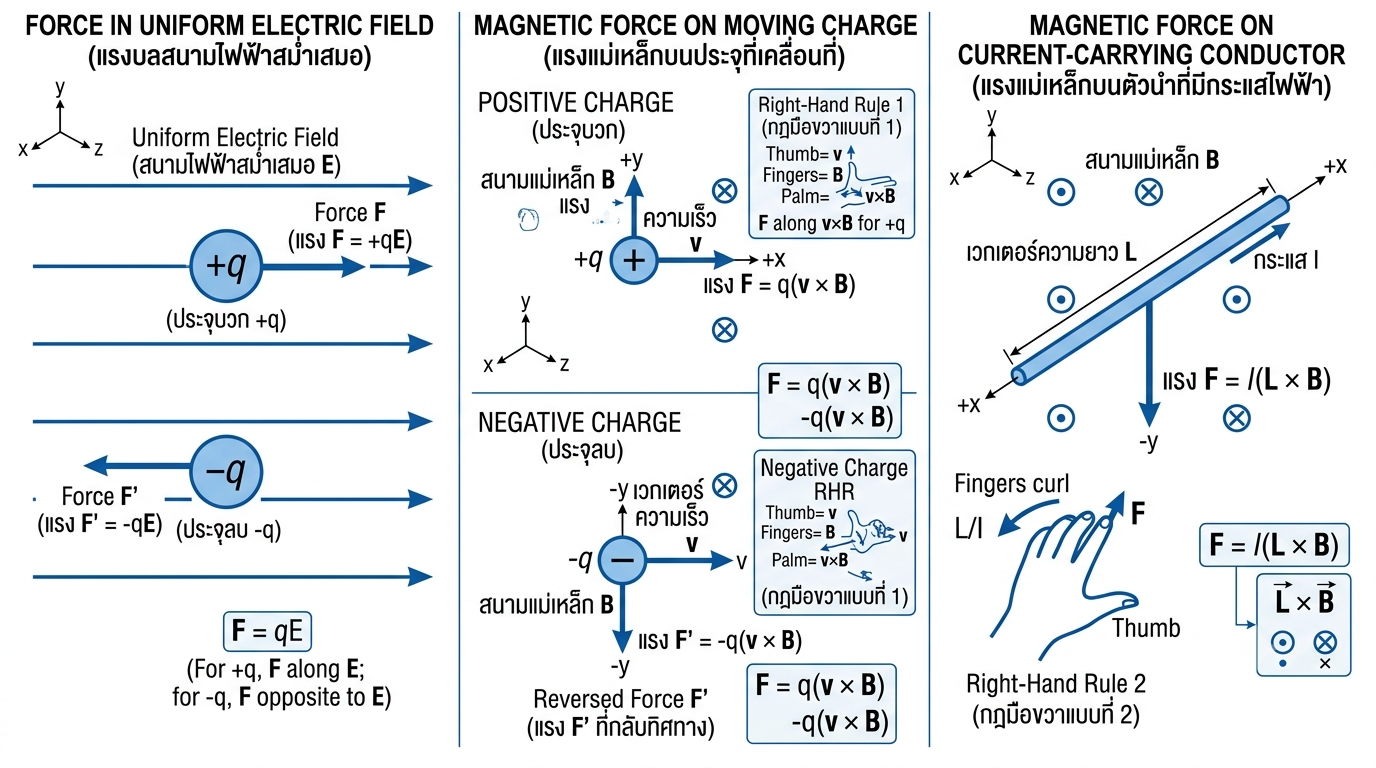
\includegraphics[width=0.8\textwidth]{images/chapter3/figure-08.png}
    \caption{ทิศแรงไฟฟ้าและแรงแม่เหล็กบนประจุและตัวนำ}
\end{figure}

\subsection{8. ความเข้าใจผิดที่พบบ่อย}

\subsubsection{8.1 เวกเตอร์ ``เป็นลบ''}

เวกเตอร์ตรงข้ามเขียนเป็น \(-\mathbf{A}\) มีขนาดเท่าเดิมและทิศกลับกัน องค์ประกอบบางแกนอาจติดลบตามทิศอ้างอิง แต่ขนาดเวกเตอร์ไม่เป็นลบ

\subsubsection{8.2 ขนาดเวกเตอร์เท่ากับผลบวกองค์ประกอบ}

ไม่ถูกต้อง ต้องใช้

\[
|\mathbf{A}|=\sqrt{A_x^2+A_y^2+A_z^2}
\]

\subsubsection{8.3 ดอตและครอสใช้แทนกันได้}

ดอตให้สเกลาร์และเลือกองค์ประกอบตามแนว ครอสให้เวกเตอร์ตั้งฉาก การเลือกผิดทำให้ชนิด หน่วย และความหมายของคำตอบผิด

\subsubsection{8.4 ครอสโปรดักต์สลับที่}

ไม่จริง

\[
\mathbf{A}\times\mathbf{B}=-(\mathbf{B}\times\mathbf{A})
\]

\subsubsection{8.5 ไดเวอร์เจนซ์เป็นเวกเตอร์}

ไดเวอร์เจนซ์ให้สเกลาร์ เคิร์ลให้เวกเตอร์ และเกรเดียนต์ของสเกลาร์ให้เวกเตอร์

\subsubsection{8.6 ไดเวอร์เจนซ์ศูนย์หมายถึงสนามศูนย์}

ไม่จริง สนามอาจมีค่าและหมุนวนได้โดยไม่มีฟลักซ์ออกสุทธิ

\subsubsection{8.7 เคิร์ลศูนย์ทำให้อินทิกรัลรอบเส้นปิดเป็นศูนย์เสมอ}

ต้องพิจารณาโดเมนและจุดเอกฐานด้วย หากบริเวณไม่เป็น simply connected อาจต้องวิเคราะห์เพิ่มเติม

\subsubsection{8.8 ฐานทรงกระบอกคงทิศ}

\(\mathbf{a}_\rho\) และ \(\mathbf{a}_\phi\) เปลี่ยนทิศตาม \(\phi\) จึงห้ามใช้กฎอนุพันธ์เหมือนฐานฉากโดยไม่ตรวจ scale factor

\subsubsection{8.9 สนามแม่เหล็กทำงานโดยตรงต่อประจุ}

เพราะ \(\mathbf{F}_m\perp\mathbf{v}\) จึงมี \(\mathbf{F}_m\cdot\mathbf{v}=0\) ในกรณีอุดมคติ สนามแม่เหล็กเปลี่ยนทิศความเร็วได้แต่ไม่เปลี่ยนพลังงานจลน์โดยตรง

\subsubsection{8.10 เส้นสนามเป็นวัตถุจริง}

เส้นสนามเป็นเครื่องมือแสดงทิศและขนาดสัมพัทธ์ ไม่ใช่วัตถุหรือเส้นทางบังคับของอนุภาคทุกกรณี

\subsection{9. การประยุกต์ใช้ในงานจริง}

\subsubsection{9.1 การออกแบบฉนวนและอิเล็กโทรด}

เกรเดียนต์ของศักย์ใช้ประเมินสนามไฟฟ้า บริเวณมุมแหลมหรือรัศมีโค้งเล็กอาจมีสนามเข้มสูง จึงต้องปรับรูปทรงและระยะฉนวนเพื่อลดความเสี่ยงการคายประจุ

\subsubsection{9.2 สายโคแอกเชียลและสายส่ง}

สมมาตรทรงกระบอกทำให้สนามไฟฟ้าอยู่ตาม \(\mathbf{a}_\rho\) และสนามแม่เหล็กอยู่ตาม \(\mathbf{a}_\phi\) การเลือกพิกัดที่เหมาะสมลดความซับซ้อนของสมการ

\subsubsection{9.3 มอเตอร์ไฟฟ้าและแอคชูเอเตอร์}

แรง \(I\mathbf{L}\times\mathbf{B}\) เป็นพื้นฐานของการสร้างแรงและแรงบิดในมอเตอร์ ลำโพง และขดลวดเคลื่อนที่

\subsubsection{9.4 เซนเซอร์ฮอลล์}

ค่าที่เซนเซอร์วัดได้สัมพันธ์กับองค์ประกอบของ \(\mathbf{B}\) ตามแกนไวรับ จึงตีความเป็นการฉายด้วยดอตโปรดักต์

\subsubsection{9.5 EMC และการเชื่อมโยงสนาม}

แนวคิดเคิร์ลช่วยอธิบายสนามที่เกิดจากกระแสเปลี่ยนตามเวลา การเหนี่ยวนำระหว่างลูป และเหตุผลที่ควรลดพื้นที่ลูปกระแสและออกแบบเส้นทางกระแสกลับ

\subsubsection{9.6 การวิเคราะห์เชิงตัวเลข}

เมื่อรูปทรงซับซ้อน วิศวกรใช้วิธี Finite Element หรือ Finite Difference แม้ซอฟต์แวร์จะคำนวณให้ ผู้ใช้ยังต้องเลือกพิกัด เงื่อนไขขอบเขต ตรวจหน่วย และตีความเวกเตอร์อย่างถูกต้อง

\subsection{10. กิจกรรมการเรียนรู้ระหว่างเรียน}

\subsubsection{กิจกรรมที่ 1: จำแนกปริมาณและอธิบายเหตุผล}

\begin{itemize}
\item \textbf{CLO:} CLO1
\item \textbf{เวลา:} 15 นาที
\item \textbf{รูปแบบ:} กลุ่ม 3--4 คน
\item \textbf{สื่อ:} บัตรคำ เช่น ศักย์ สนามไฟฟ้า พลังงาน ความหนาแน่นกระแส
\item \textbf{ขั้นตอน:} แบ่งบัตรเป็นสเกลาร์ เวกเตอร์ สนามสเกลาร์ และสนามเวกเตอร์ แล้วเขียนเหตุผลหนึ่งประโยค
\item \textbf{ผลที่คาดหวัง:} จำแนกจากจำนวนองค์ประกอบและการขึ้นกับตำแหน่ง
\item \textbf{ประเมิน:} ความถูกต้องและคุณภาพของเหตุผล
\end{itemize}

\subsubsection{กิจกรรมที่ 2: เลือกระบบพิกัดจากสมมาตร}

\begin{itemize}
\item \textbf{CLO:} CLO2
\item \textbf{เวลา:} 20 นาที
\item \textbf{รูปแบบ:} คู่
\item \textbf{สื่อ:} ภาพแผ่นขนาน ลวดตรง สายโคแอกเชียล ทรงกลม และอิเล็กโทรดซับซ้อน
\item \textbf{ขั้นตอน:} ระบุสมมาตร เลือกพิกัด และบอกว่าปริมาณน่าจะขึ้นกับตัวแปรใด
\item \textbf{ประเมิน:} เลือกพิกัดถูก ระบุตัวแปรถูก และอธิบายสมมาตรชัดเจน
\end{itemize}

\subsubsection{กิจกรรมที่ 3: คลินิกกฎมือขวา}

\begin{itemize}
\item \textbf{CLO:} CLO3, CLO5
\item \textbf{เวลา:} 20 นาที
\item \textbf{รูปแบบ:} รายบุคคลแล้วตรวจเป็นคู่
\item \textbf{ขั้นตอน:} วิเคราะห์ทิศครอสโปรดักต์ 4 กรณี และเพิ่มกรณีประจุลบ 2 กรณี
\item \textbf{ผลที่คาดหวัง:} ลดการสลับลำดับและการลืมกลับทิศสำหรับประจุลบ
\item \textbf{ประเมิน:} คำตอบพร้อมเหตุผลสั้น
\end{itemize}

\subsubsection{กิจกรรมที่ 4: วิเคราะห์ภาพสนามด้วย Grad--Div--Curl}

\begin{itemize}
\item \textbf{CLO:} CLO4
\item \textbf{เวลา:} 25 นาที
\item \textbf{รูปแบบ:} กลุ่ม
\item \textbf{ขั้นตอน:} ทำนายเครื่องหมายไดเวอร์เจนซ์ ทิศเคิร์ล สร้างฟังก์ชันอย่างง่าย และคำนวณตรวจสอบ
\item \textbf{ผลที่คาดหวัง:} เชื่อมภาพเชิงคุณภาพกับอนุพันธ์เชิงปริมาณ
\item \textbf{ประเมิน:} ความสอดคล้องระหว่างคำทำนาย ฟังก์ชัน และผลคำนวณ
\end{itemize}

\newpage

\subsection{11. กิจกรรมปฏิบัติการ}

\subsubsection{กิจกรรมปฏิบัติการที่ 1: การทำแผนที่ศักย์ไฟฟ้าบนกระดาษนำไฟฟ้า}

\paragraph{1. วัตถุประสงค์}

ผู้เรียนสามารถวัดศักย์ วาดเส้นศักย์เท่ากัน ประมาณสนามจาก \(\mathbf{E}=-\nabla V\) เปรียบเทียบรูปอิเล็กโทรด และอภิปรายความคลาดเคลื่อนได้

\paragraph{2. หลักการ}

ในแบบจำลองสองมิติ เส้นสนามตั้งฉากกับเส้นศักย์ และประมาณองค์ประกอบสนามได้ด้วย

\[
E_s\approx-\frac{\Delta V}{\Delta s}
\]

\paragraph{3. อุปกรณ์}

\begin{itemize}
\item แหล่งจ่าย DC 0--12 V ตั้งใช้งานไม่เกิน 10 V และจำกัดกระแส
\item กระดาษนำไฟฟ้าหรือชุดแผ่นนำไฟฟ้า
\item อิเล็กโทรดแผ่นขนานและจุด--แผ่น
\item ดิจิทัลมัลติมิเตอร์ความต้านทานอินพุตสูง
\item สายหุ้มฉนวน ไม้บรรทัด และกระดาษกราฟ
\item คอมพิวเตอร์พร้อม Python/MATLAB/Octave เป็นตัวเลือก
\end{itemize}

\paragraph{4. แผนภาพ}

% [รูปที่ 9: ชุดทดลองทำแผนที่ศักย์ไฟฟ้าบนกระดาษนำไฟฟ้า]
% ประเภทภาพ: Experimental Setup
% ตำแหน่งที่แนะนำ: หัวข้อกิจกรรมปฏิบัติการ ข้อ 4
% วัตถุประสงค์การเรียนรู้: แสดงการต่ออุปกรณ์แรงดันต่ำอย่างปลอดภัย
% คำอธิบายภาพ: แหล่งจ่าย 0–10 VDC ต่อกับอิเล็กโทรดบนแผ่นนำไฟฟ้า ขั้ว COM ต่อกับขั้วอ้างอิงและใช้โพรบวัดตามตาราง
% องค์ประกอบที่ต้องมี: แหล่งจ่ายจำกัดกระแส แผ่นนำไฟฟ้า มัลติมิเตอร์ โพรบ และเส้นศักย์ตัวอย่าง
% ภาษาของป้ายกำกับ: ไทยและอังกฤษ
% สัดส่วนภาพ: 16:9
% Image Generation Prompt: Safe educational laboratory setup for mapping electric potential on conductive paper. Show a current-limited 0–10 VDC supply connected to two electrodes on a gridded conductive sheet, digital multimeter COM connected to the zero-volt reference electrode, movable probe sampling grid points, example equipotential contours and electric-field arrows perpendicular to contours. White background, Thai-English labels, 16:9.
% Alt Text: ชุดทดลองแรงดันต่ำสำหรับวัดศักย์และประมาณสนามบนแผ่นนำไฟฟ้า

\begin{figure}[htbp]
    \centering
    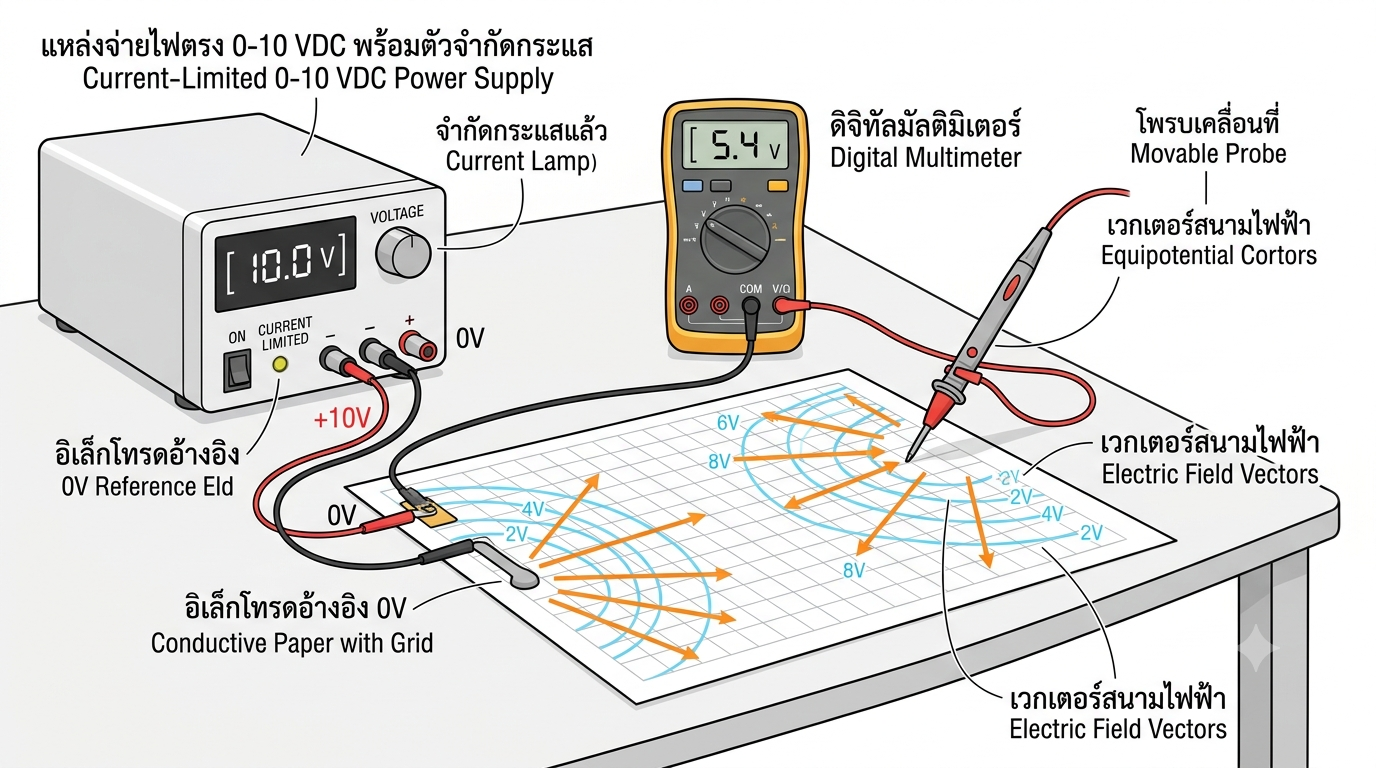
\includegraphics[width=0.8\textwidth]{images/chapter3/figure-09.png}
    \caption{ชุดทดลองทำแผนที่ศักย์ไฟฟ้าบนกระดาษนำไฟฟ้า}
\end{figure}

\paragraph{5. ความปลอดภัย}

\begin{enumerate}
\item ใช้แรงดันไม่เกิน 10 VDC และจำกัดกระแส
\item ปิดแหล่งจ่ายก่อนเปลี่ยนอิเล็กโทรดหรือสาย
\item ห้ามใช้ไฟบ้านหรือแหล่งจ่ายที่ไม่แยกทางไฟฟ้า
\item ตรวจฉนวนสายและรักษาพื้นที่ให้แห้ง
\item ไม่กดโพรบแรงจนแผ่นเสียหาย
\end{enumerate}

\paragraph{6. ขั้นตอน}

\begin{enumerate}
\item ตั้งแหล่งจ่ายเป็นศูนย์และปิดสวิตช์
\item ติดตั้งอิเล็กโทรดแผ่นขนานและต่อ 0 V กับ 10 V
\item ต่อ COM ของมัลติมิเตอร์กับขั้วอ้างอิง
\item วัดศักย์ตามจุดตารางโดยไม่แต่งค่าที่ไม่ได้วัด
\item ทำเครื่องหมายจุดใกล้ 2, 4, 6 และ 8 V แล้วลากเส้นศักย์
\item วาดลูกศรสนามตั้งฉากและชี้จากศักย์สูงไปต่ำ
\item ประมาณ \(|E|\approx|\Delta V/\Delta s|\) อย่างน้อยสามตำแหน่ง
\item ปิดแหล่งจ่าย เปลี่ยนเป็นอิเล็กโทรดจุด--แผ่น และทำซ้ำ
\item เปรียบเทียบสนามบริเวณกลาง ขอบ และใกล้ปลายแหลม
\end{enumerate}

\paragraph{7. ตารางบันทึกผล}

\begin{table}[htbp]
    \centering
    \begin{tabular}{l r r r r r l}
        \hline
        \textbf{รูปแบบอิเล็กโทรด} & \textbf{จุด \((x,y)\) cm} & \textbf{ศักย์ (V)} & \textbf{\(\Delta V\) (V)} & \textbf{\(\Delta s\) (m)} & \textbf{\(|E|\) (V/m)} & \textbf{หมายเหตุ} \\
        \hline
        แผ่นขนาน &  &  &  &  &  &  \\
        แผ่นขนาน &  &  &  &  &  &  \\
        จุด--แผ่น &  &  &  &  &  &  \\
        จุด--แผ่น &  &  &  &  &  &  \\
        \hline
    \end{tabular}
\end{table}

\paragraph{8. วิเคราะห์ผล}

\begin{itemize}
\item เส้นศักย์ใกล้กันหมายถึงขนาดสนามสูงกว่า
\item บริเวณกลางแผ่นขนานควรมีสนามค่อนข้างสม่ำเสมอ
\item บริเวณขอบเกิด fringing field
\item ใกล้ปลายแหลมเส้นศักย์มักหนาแน่น
\item ความคลาดเคลื่อนมาจากความต้านทานสัมผัส ความละเอียดตาราง ตำแหน่งโพรบ และความไม่สม่ำเสมอของแผ่น
\end{itemize}

\paragraph{9. คำถามหลังทดลอง}

\begin{enumerate}
\item เหตุใดเส้นสนามตั้งฉากกับเส้นศักย์
\item บริเวณใดมีสนามสูงสุด และข้อมูลใดสนับสนุน
\item รูปทรงอิเล็กโทรดมีผลอย่างไร
\item การกลับขั้วทำให้รูปและทิศสนามเปลี่ยนอย่างไร
\item แบบจำลองสองมิตินี้มีข้อจำกัดอะไร
\end{enumerate}

\paragraph{10. เกณฑ์ประเมิน}

\begin{table}[htbp]
    \centering
    \begin{tabularx}{0.76\textwidth}{Y r}
        \hline
        \textbf{ด้าน} & \textbf{สัดส่วน} \\
        \hline
        ความปลอดภัยและการต่ออุปกรณ์ & 20\% \\
        การบันทึกข้อมูลและหน่วย & 20\% \\
        แผนที่ศักย์ & 20\% \\
        การประมาณสนาม & 20\% \\
        การอภิปรายข้อจำกัดและความคลาดเคลื่อน & 20\% \\
        \hline
    \end{tabularx}
\end{table}

\subsection{12. การใช้ซอฟต์แวร์ โค้ด และการจำลอง}

\subsubsection{12.1 วัตถุประสงค์}

\begin{enumerate}
\item สร้างภาพสนามเวกเตอร์เพื่อช่วยตีความทิศและขนาด
\item สร้างเส้นชั้นศักย์และตรวจว่าทิศเกรเดียนต์ตั้งฉากกับเส้นชั้นค่า
\item คำนวณเชิงสัญลักษณ์ของเกรเดียนต์ ไดเวอร์เจนซ์ และเคิร์ล
\item เปรียบเทียบผลซอฟต์แวร์กับการคำนวณด้วยมือ
\item ตรวจจุดเอกฐาน โดเมน และข้อจำกัดของภาพที่สร้าง
\end{enumerate}

\subsubsection{12.2 เครื่องมือ}

\begin{itemize}
\item Python 3 พร้อม NumPy, Matplotlib และ SymPy
\item หรือ MATLAB/GNU Octave ที่มีคำสั่ง \texttt{meshgrid}, \texttt{quiver}, \texttt{contour}
\end{itemize}

ไม่รับรองความเข้ากันได้ทุกเวอร์ชัน ผู้เรียนควรตรวจเอกสารของรุ่นซอฟต์แวร์ที่ใช้

\subsubsection{12.3 Python: เส้นศักย์และสนามไฟฟ้า}

กำหนด

\[
V(x,y)=10-2x^2-y^2
\]

ดังนั้น

\[
\mathbf{E}=-\nabla V=4x\mathbf{a}_x+2y\mathbf{a}_y
\]

\begin{verbatim}
import numpy as np
import matplotlib.pyplot as plt

x = np.linspace(-2.0, 2.0, 21)
y = np.linspace(-2.0, 2.0, 21)
X, Y = np.meshgrid(x, y)

V = 10.0 - 2.0 * X**2 - Y**2
Ex = 4.0 * X
Ey = 2.0 * Y

magnitude = np.hypot(Ex, Ey)
nonzero = magnitude > 0

Ex_unit = np.zeros_like(Ex)
Ey_unit = np.zeros_like(Ey)
Ex_unit[nonzero] = Ex[nonzero] / magnitude[nonzero]
Ey_unit[nonzero] = Ey[nonzero] / magnitude[nonzero]

plt.figure(figsize=(9, 6))
contours = plt.contour(X, Y, V, levels=10)
plt.clabel(contours, inline=True, fontsize=8)
plt.quiver(X, Y, Ex_unit, Ey_unit, magnitude)
plt.xlabel("x (m)")
plt.ylabel("y (m)")
plt.title("Equipotential contours and electric-field direction")
plt.axis("equal")
plt.tight_layout()
plt.show()
\end{verbatim}

\paragraph{อธิบายโค้ด}

\begin{itemize}
\item \texttt{meshgrid} สร้างจุดตัวอย่างบนระนาบ
\item \texttt{contour} สร้างเส้นศักย์เท่ากัน
\item \texttt{quiver} แสดงลูกศรสนาม
\item normalization ใช้เปรียบเทียบทิศ ส่วน \texttt{magnitude} ใช้บอกความเข้มสัมพัทธ์
\item จุด \((0,0)\) มีสนามศูนย์ จึงต้องป้องกันการหารศูนย์
\end{itemize}

\paragraph{ผลที่ควรสังเกต}

\begin{enumerate}
\item ลูกศรสนามตั้งฉากกับเส้นศักย์
\item สนามชี้ไปทางศักย์ลดลง
\item ขนาดสนามเพิ่มเมื่อ \(|x|\) หรือ \(|y|\) เพิ่ม
\item การทำลูกศรให้ยาวเท่ากันช่วยดูทิศ แต่ไม่ควรตีความว่าแสดงขนาดจริง
\end{enumerate}

\subsubsection{12.4 SymPy: ตรวจ Grad--Div--Curl}

\begin{verbatim}
import sympy as sp

x, y, z = sp.symbols("x y z", real=True)

V = 10 - 2*x**2 - y**2 - 3*z
grad_V = sp.Matrix([
    sp.diff(V, x),
    sp.diff(V, y),
    sp.diff(V, z),
])

A = sp.Matrix([-y, x, 0])

div_A = (
    sp.diff(A[0], x)
    + sp.diff(A[1], y)
    + sp.diff(A[2], z)
)

curl_A = sp.Matrix([
    sp.diff(A[2], y) - sp.diff(A[1], z),
    sp.diff(A[0], z) - sp.diff(A[2], x),
    sp.diff(A[1], x) - sp.diff(A[0], y),
])

print("grad(V) =", grad_V)
print("div(A) =", sp.simplify(div_A))
print("curl(A) =", curl_A)
\end{verbatim}

ผลที่คาดหวัง:

\[
\nabla V=(-4x,-2y,-3)
\]

\[
\nabla\cdot\mathbf{A}=0
\]

\[
\nabla\times\mathbf{A}=(0,0,2)
\]

\subsubsection{12.5 MATLAB/GNU Octave}

\begin{verbatim}
[x, y] = meshgrid(linspace(-2, 2, 21), linspace(-2, 2, 21));

V  = 10 - 2*x.^2 - y.^2;
Ex = 4*x;
Ey = 2*y;

figure;
contour(x, y, V, 10);
hold on;
quiver(x, y, Ex, Ey);
axis equal;
xlabel('x (m)');
ylabel('y (m)');
title('Equipotential contours and electric field');
grid on;
\end{verbatim}

\subsubsection{12.6 งานมอบหมายซอฟต์แวร์}

ให้เลือกหนึ่งสนาม

\begin{enumerate}
\item \(\mathbf{A}=x\mathbf{a}_x+y\mathbf{a}_y\)
\item \(\mathbf{A}=-y\mathbf{a}_x+x\mathbf{a}_y\)
\item \(\mathbf{A}=\dfrac{x\mathbf{a}_x+y\mathbf{a}_y}{x^2+y^2}\) โดยตัดจุดกำเนิดออก
\end{enumerate}

ดำเนินการดังนี้

\begin{itemize}
\item สร้าง quiver plot
\item ทำนายไดเวอร์เจนซ์และเคิร์ลจากภาพ
\item คำนวณเชิงสัญลักษณ์
\item อธิบายความสอดคล้องระหว่างภาพกับผลคำนวณ
\item ระบุจุดเอกฐานและข้อจำกัดของโดเมน
\item เปลี่ยนช่วงแกนหรือความละเอียดกริด แล้วอธิบายผลต่อการมองเห็น
\end{itemize}

% [รูปที่ 10: ตัวอย่างเส้นศักย์และสนามไฟฟ้าจากซอฟต์แวร์]
% ประเภทภาพ: Graph
% ตำแหน่งที่แนะนำ: หลังหัวข้อ 12.6
% วัตถุประสงค์การเรียนรู้: แสดงความตั้งฉากระหว่างเส้นศักย์กับสนาม
% คำอธิบายภาพ: กราฟระนาบ $xy$ มี contour ของ $V=10-2x^2-y^2$ และลูกศร $\mathbf{E}=(4x,2y)$
% องค์ประกอบที่ต้องมี: แกนพร้อมหน่วย เส้น contour มีค่ากำกับ ลูกศรสนาม และ colorbar ขนาดสนาม
% ภาษาของป้ายกำกับ: ไทยและอังกฤษ
% สัดส่วนภาพ: 4:3
% Graph Generation Prompt: Plot V(x,y)=10-2x^2-y^2 over -2<=x<=2 and -2<=y<=2 with labeled contour lines. Overlay E=-grad(V)=(4x,2y) using quiver arrows. Use equal axis scaling, axes in meters, a colorbar for field magnitude, and clearly show arrows normal to equipotential contours. Academic engineering graph, white background.
% Alt Text: เส้นศักย์รูปวงรีและลูกศรสนามไฟฟ้าที่ตั้งฉากกับเส้นศักย์

\begin{figure}[htbp]
    \centering
    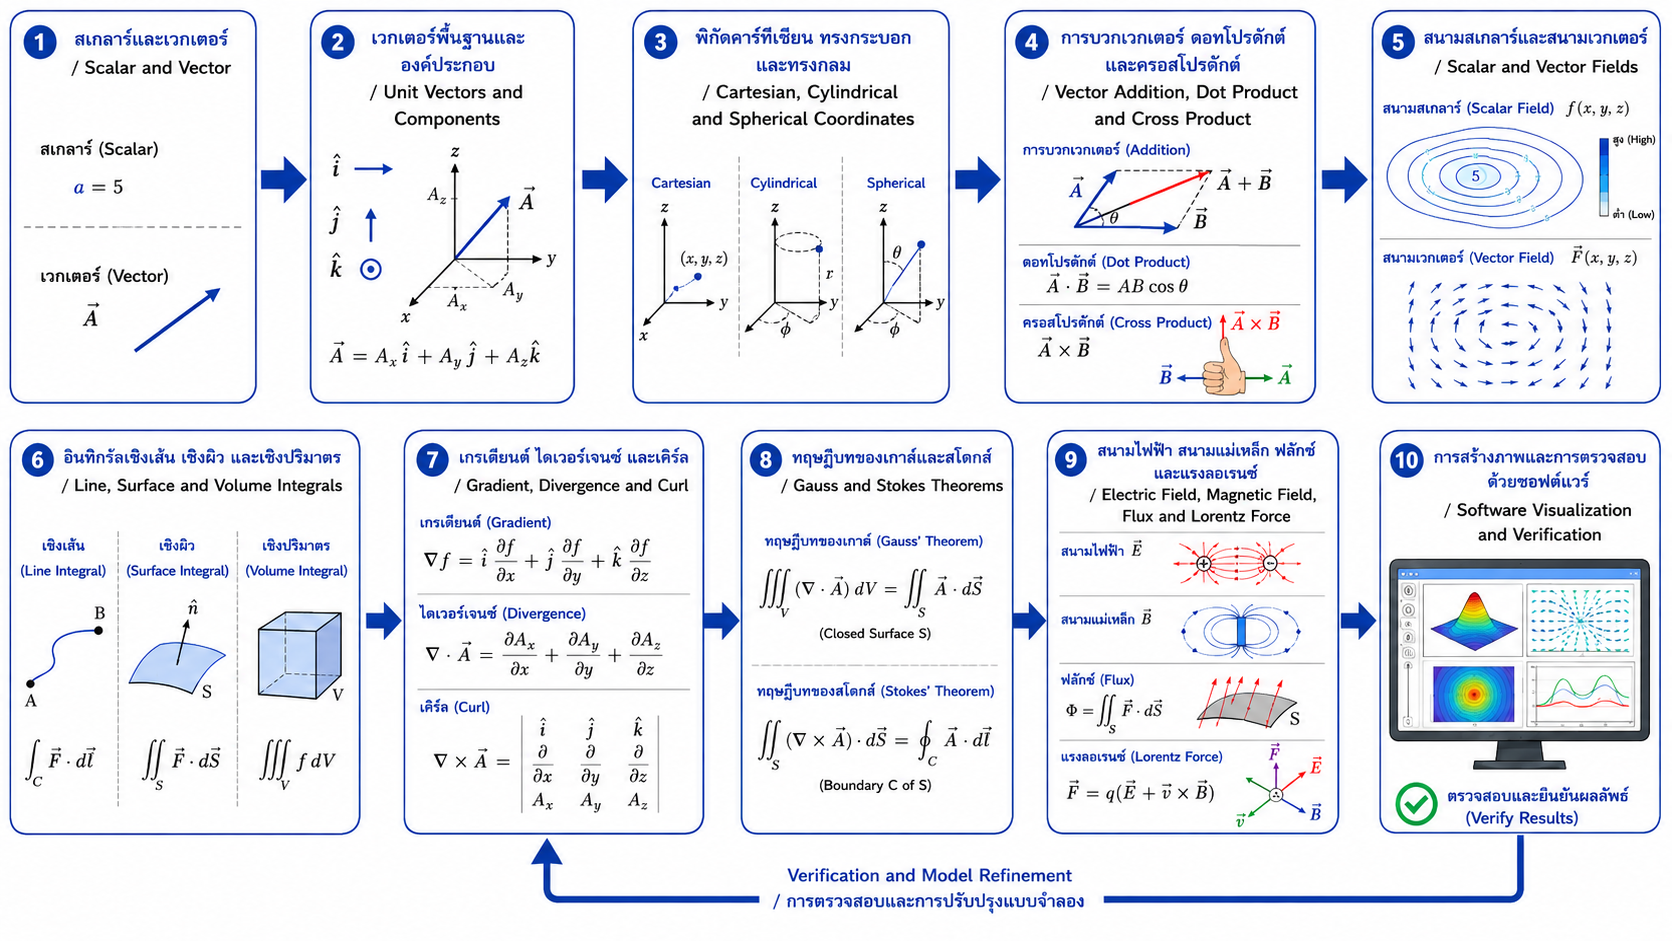
\includegraphics[width=0.8\textwidth]{images/chapter3/figure-01.png}
    \caption{ตัวอย่างเส้นศักย์และสนามไฟฟ้าจากซอฟต์แวร์}
\end{figure}

\subsubsection{12.7 ข้อผิดพลาดที่พบบ่อยในการใช้ซอฟต์แวร์}

\begin{itemize}
\item ลืมเครื่องหมายลบใน \(\mathbf{E}=-\nabla V\)
\item ลืมใช้ \texttt{.*}, \texttt{.\^{}} ใน MATLAB/Octave สำหรับข้อมูลแบบอาร์เรย์
\item กริดหยาบเกินไปจนภาพไม่สะท้อนลักษณะสนาม
\item สเกลแกนไม่เท่ากัน ทำให้ทิศดูบิดเบือน
\item ใช้ normalization แล้วตีความขนาดผิด
\item รวมจุดเอกฐานไว้ในกริด ทำให้เกิด \texttt{inf} หรือ \texttt{nan}
\item เชื่อผลซอฟต์แวร์โดยไม่ตรวจหน่วยและกรณีง่ายด้วยมือ
\end{itemize}

\subsection{13. สรุปท้ายบท}

\begin{enumerate}
\item สเกลาร์มีขนาด ส่วนเวกเตอร์มีทั้งขนาดและทิศทาง
\item เวกเตอร์เขียนเป็นองค์ประกอบตามเวกเตอร์หนึ่งหน่วย และขนาดหาได้จากผลบวกกำลังสองขององค์ประกอบ
\item พิกัดฉากเหมาะกับสมมาตรตามระนาบ พิกัดทรงกระบอกเหมาะกับสมมาตรรอบแกน และพิกัดทรงกลมเหมาะกับสมมาตรรอบจุด
\item ดอตโปรดักต์ให้สเกลาร์ ใช้กับการฉาย งาน และฟลักซ์
\item ครอสโปรดักต์ให้เวกเตอร์ตั้งฉาก ใช้กับพื้นที่ แรงแม่เหล็ก และแรงบนตัวนำ
\item สนามสเกลาร์ให้ค่าหนึ่งค่าต่อจุด ส่วนสนามเวกเตอร์ให้เวกเตอร์ต่อจุด
\item เกรเดียนต์ชี้ไปทางเพิ่มเร็วที่สุด และ \(\mathbf{E}=-\nabla V\)
\item ไดเวอร์เจนซ์บอกการแผ่ออกสุทธิ ส่วนเคิร์ลบอกการหมุนวนเฉพาะที่
\item ทฤษฎีบทไดเวอร์เจนซ์เชื่อมฟลักซ์ผ่านผิวปิดกับแหล่งกำเนิดในปริมาตร
\item ทฤษฎีบทสโตกส์เชื่อมการไหลเวียนรอบเส้นขอบกับเคิร์ลผ่านพื้นผิว
\item กฎสนามแม่เหล็กไฟฟ้าใช้ภาษาเวกเตอร์เพื่อเชื่อมประจุ กระแส สนาม และการเปลี่ยนตามเวลา
\item ซอฟต์แวร์ช่วยสร้างภาพและตรวจผล แต่ผู้เรียนต้องตรวจสมมาตร หน่วย ทิศ โดเมน และจุดเอกฐาน
\end{enumerate}

\subsubsection{13.1 ตารางสมการสำคัญ}

\begin{table}[htbp]
    \centering
    \begin{tabular}{l l}
        \hline
        \textbf{หัวข้อ} & \textbf{สมการ} \\
        \hline
        ขนาดเวกเตอร์ & \(|\mathbf{A}|=\sqrt{A_x^2+A_y^2+A_z^2}\) \\
        เวกเตอร์หนึ่งหน่วย & \(\mathbf{a}_A=\mathbf{A}/|\mathbf{A}|\) \\
        ดอตโปรดักต์ & \(\mathbf{A}\cdot\mathbf{B}=|\mathbf{A}||\mathbf{B}|\cos\theta\) \\
        ครอสโปรดักต์ & \(\mathbf{A}\times\mathbf{B}=|\mathbf{A}||\mathbf{B}|\sin\theta\,\mathbf{a}_n\) \\
        งาน & \(W=\int_C\mathbf{F}\cdot d\mathbf{l}\) \\
        ฟลักซ์ & \(\Phi=\int_S\mathbf{A}\cdot d\mathbf{S}\) \\
        สนามไฟฟ้าจากศักย์ & \(\mathbf{E}=-\nabla V\) \\
        ไดเวอร์เจนซ์ & \(\nabla\cdot\mathbf{A}\) \\
        เคิร์ล & \(\nabla\times\mathbf{A}\) \\
        ทฤษฎีบทไดเวอร์เจนซ์ & \(\oint_S\mathbf{A}\cdot d\mathbf{S}=\int_V\nabla\cdot\mathbf{A}\,dV\) \\
        ทฤษฎีบทสโตกส์ & \(\oint_C\mathbf{A}\cdot d\mathbf{l}=\int_S(\nabla\times\mathbf{A})\cdot d\mathbf{S}\) \\
        แรงลอเรนซ์ & \(\mathbf{F}=q(\mathbf{E}+\mathbf{v}\times\mathbf{B})\) \\
        แรงบนตัวนำ & \(\mathbf{F}=I\mathbf{L}\times\mathbf{B}\) \\
        \hline
    \end{tabular}
\end{table}

\subsection{14. คำถามทบทวน}

\begin{enumerate}
\item เพราะเหตุใดสนามไฟฟ้าจึงเป็นเวกเตอร์ แต่ศักย์ไฟฟ้าเป็นสเกลาร์
\item การเลือกระบบพิกัดจากสมมาตรช่วยลดความซับซ้อนอย่างไร
\item เปรียบเทียบดอตโปรดักต์กับครอสโปรดักต์ทั้งชนิดผลลัพธ์และการใช้งาน
\item เหตุใดสนามไฟฟ้าสถิตตั้งฉากกับพื้นผิวศักย์เท่ากัน
\item ไดเวอร์เจนซ์เป็นศูนย์บอกอะไรและไม่ได้บอกอะไร
\item เคิร์ลสัมพันธ์กับทฤษฎีบทสโตกส์อย่างไร
\item เหตุใดแรงแม่เหล็กเพียงอย่างเดียวไม่เปลี่ยนพลังงานจลน์ของประจุ
\item เปรียบเทียบกฎของเกาส์รูปอินทิกรัลกับรูปอนุพันธ์
\item จุดเอกฐานมีผลต่อการใช้ตัวดำเนินการเวกเตอร์อย่างไร
\item การสร้างภาพด้วยซอฟต์แวร์มีประโยชน์และข้อจำกัดอะไร
\end{enumerate}

\subsection{15. แบบฝึกหัดท้ายบท}

\subsubsection{15.1 ระดับพื้นฐาน}

\begin{enumerate}
\item จำแนกปริมาณต่อไปนี้เป็นสเกลาร์หรือเวกเตอร์: ศักย์ไฟฟ้า พลังงาน สนามไฟฟ้า ความหนาแน่นกระแส และกำลังไฟฟ้า
\item ให้ \(\mathbf{A}=4\mathbf{a}_x-3\mathbf{a}_y+12\mathbf{a}_z\) จงหาขนาดและเวกเตอร์หนึ่งหน่วย
\item จุด \(P=(6,-8,3)\) จงแปลงเป็นพิกัดทรงกระบอก โดยใช้มุมช่วง \(0^\circ\) ถึง \(360^\circ\)
\item ให้ \(\mathbf{A}=2\mathbf{a}_x+3\mathbf{a}_y-\mathbf{a}_z\) และ \(\mathbf{B}=-\mathbf{a}_x+4\mathbf{a}_y+2\mathbf{a}_z\) จงหา \(\mathbf{A}+\mathbf{B}\) และ \(\mathbf{A}-\mathbf{B}\)
\item ให้ \(\mathbf{A}=3\mathbf{a}_x+4\mathbf{a}_y\) และ \(\mathbf{B}=4\mathbf{a}_x-3\mathbf{a}_y\) จงหา \(\mathbf{A}\cdot\mathbf{B}\) และมุมระหว่างเวกเตอร์
\end{enumerate}

\subsubsection{15.2 ระดับวิเคราะห์}

\begin{enumerate}
\setcounter{enumi}{5}
\item ให้ \(P_1=(1,-2,3)\) และ \(P_2=(5,1,-1)\) จงหาเวกเตอร์ ระยะทาง และเวกเตอร์หนึ่งหน่วยจาก \(P_1\) ไป \(P_2\)
\item ให้ \(\mathbf{A}=2\mathbf{a}_x-\mathbf{a}_y+2\mathbf{a}_z\) และ \(\mathbf{B}=\mathbf{a}_x+2\mathbf{a}_y-2\mathbf{a}_z\) จงหามุมระหว่างเวกเตอร์
\item หา \(\mathbf{A}\times\mathbf{B}\) เมื่อ \(\mathbf{A}=\mathbf{a}_x+2\mathbf{a}_y+3\mathbf{a}_z\) และ \(\mathbf{B}=2\mathbf{a}_x-\mathbf{a}_y+\mathbf{a}_z\) แล้วตรวจว่าผลลัพธ์ตั้งฉากกับทั้งสองเวกเตอร์
\item ให้ \(V=5x^2-2xy+z^2\) V จงหา \(\nabla V\) และ \(\mathbf{E}\) ที่ \((1,2,-1)\)
\item ให้ \(\mathbf{A}=xy\mathbf{a}_x+yz\mathbf{a}_y+zx\mathbf{a}_z\) จงหาไดเวอร์เจนซ์ที่ \((1,2,3)\)
\item ให้ \(\mathbf{A}=z\mathbf{a}_x+x\mathbf{a}_y+y\mathbf{a}_z\) จงหาเคิร์ล
\item ให้ \(\mathbf{F}=2x\mathbf{a}_x+2y\mathbf{a}_y\) N จงหางานจาก \((0,0)\) ไป \((2,1)\) และอธิบายว่าเหตุใดไม่ขึ้นกับเส้นทาง
\item สนามสม่ำเสมอ \(\mathbf{A}=5\mathbf{a}_z\) ผ่านพื้นผิวพื้นที่ \(0.20\) m\(^2\) ซึ่งเวกเตอร์ปกติทำมุม \(60^\circ\) กับ \(+z\) จงหาฟลักซ์
\end{enumerate}

\subsubsection{15.3 ระดับประยุกต์ใช้}

\begin{enumerate}
\setcounter{enumi}{13}
\item ประจุ \(q=3\ \mu\)C เคลื่อนที่ด้วย \(\mathbf{v}=2\times10^5\mathbf{a}_x\) m/s ใน \(\mathbf{E}=2\times10^3\mathbf{a}_y\) V/m และ \(\mathbf{B}=0.10\mathbf{a}_z\) T จงหาแรงลอเรนซ์รวม
\item ตัวนำยาว \(0.25\) m วางตาม \(\mathbf{a}_L=(3\mathbf{a}_x+4\mathbf{a}_y)/5\) มีกระแส \(8\) A ใน \(\mathbf{B}=0.50\mathbf{a}_z\) T จงหาแรง
\item ประจุ \(Q=8\) nC อยู่ที่ \(P_Q=(1,0,0)\) m จงหาสนามที่ \(P=(1,3,4)\) m ในสุญญากาศ
\item ให้ \(\mathbf{D}=4\rho\,\mathbf{a}_\rho\) nC/m\(^2\) ในทรงกระบอกรัศมี \(0.10\) m และยาว \(0.50\) m จงหาฟลักซ์ผ่านผิวด้านข้าง และอธิบายว่าผิวหัว--ท้ายมีส่วนหรือไม่
\item ออกแบบขั้นตอนเชิงคำนวณเพื่อประเมินสนามไฟฟ้าจากข้อมูลศักย์บนกริดสองมิติ ระบุวิธีประมาณอนุพันธ์ การจัดการขอบเขต และวิธีตรวจสอบผล
\end{enumerate}

\subsection{16. แนวคำตอบและเฉลยสำหรับผู้สอน}

\subsubsection{16.1 ระดับพื้นฐาน}

\paragraph{ข้อ 1}

ศักย์ไฟฟ้า พลังงาน และกำลังเป็นสเกลาร์; สนามไฟฟ้าและความหนาแน่นกระแสเป็นเวกเตอร์

\paragraph{ข้อ 2}

\[
|\mathbf{A}|=\sqrt{16+9+144}=13
\]

\[
\boxed{\mathbf{a}_A=\frac{4}{13}\mathbf{a}_x-\frac{3}{13}\mathbf{a}_y+\frac{12}{13}\mathbf{a}_z}
\]

\paragraph{ข้อ 3}

\[
\rho=\sqrt{6^2+(-8)^2}=10
\]

จุดอยู่ควอดแรนต์ที่ 4

\[
\phi=360^\circ-\tan^{-1}(8/6)=306.87^\circ
\]

\[
\boxed{(\rho,\phi,z)=(10,306.87^\circ,3)}
\]

\paragraph{ข้อ 4}

\[
\boxed{\mathbf{A}+\mathbf{B}=\mathbf{a}_x+7\mathbf{a}_y+\mathbf{a}_z}
\]

\[
\boxed{\mathbf{A}-\mathbf{B}=3\mathbf{a}_x-\mathbf{a}_y-3\mathbf{a}_z}
\]

\paragraph{ข้อ 5}

\[
\mathbf{A}\cdot\mathbf{B}=12-12=0
\]

\[
\boxed{\theta=90^\circ}
\]

\subsubsection{16.2 ระดับวิเคราะห์}

\paragraph{ข้อ 6}

\[
\mathbf{R}_{12}=4\mathbf{a}_x+3\mathbf{a}_y-4\mathbf{a}_z
\]

\[
R_{12}=\sqrt{41}\ \text{m}
\]

\[
\boxed{\mathbf{a}_{12}=\frac{4\mathbf{a}_x+3\mathbf{a}_y-4\mathbf{a}_z}{\sqrt{41}}}
\]

\paragraph{ข้อ 7}

\[
\mathbf{A}\cdot\mathbf{B}=-4,\qquad |\mathbf{A}|=|\mathbf{B}|=3
\]

\[
\boxed{\theta=\cos^{-1}(-4/9)\approx116.39^\circ}
\]

\paragraph{ข้อ 8}

\[
\boxed{\mathbf{A}\times\mathbf{B}=5\mathbf{a}_x+5\mathbf{a}_y-5\mathbf{a}_z}
\]

ตรวจสอบ:

\[
(\mathbf{A}\times\mathbf{B})\cdot\mathbf{A}=0
\]

\[
(\mathbf{A}\times\mathbf{B})\cdot\mathbf{B}=0
\]

\paragraph{ข้อ 9}

\[
\nabla V=(10x-2y)\mathbf{a}_x-2x\mathbf{a}_y+2z\mathbf{a}_z
\]

\[
\mathbf{E}=-\nabla V
\]

ที่ \((1,2,-1)\)

\[
\boxed{\mathbf{E}=-6\mathbf{a}_x+2\mathbf{a}_y+2\mathbf{a}_z\ \text{V/m}}
\]

\paragraph{ข้อ 10}

\[
\nabla\cdot\mathbf{A}=y+z+x
\]

ที่ \((1,2,3)\)

\[
\boxed{\nabla\cdot\mathbf{A}=6}
\]

\paragraph{ข้อ 11}

\[
\boxed{\nabla\times\mathbf{A}=\mathbf{a}_x+\mathbf{a}_y+\mathbf{a}_z}
\]

\paragraph{ข้อ 12}

สนามเป็นเกรเดียนต์ของ \(\psi=x^2+y^2\)

\[
W=\psi(2,1)-\psi(0,0)=5\ \text{J}
\]

\[
\boxed{W=5\ \text{J}}
\]

และ \(\nabla\times\mathbf{F}=\mathbf{0}\) ในโดเมนทั่วระนาบ จึงไม่ขึ้นกับเส้นทาง

\paragraph{ข้อ 13}

\[
\Phi=AS\cos\theta=(5)(0.20)\cos60^\circ
\]

\[
\boxed{\Phi=0.50\ \text{หน่วยสนาม}\cdot\text{m}^2}
\]

\subsubsection{16.3 ระดับประยุกต์ใช้}

\paragraph{ข้อ 14}

\[
\mathbf{v}\times\mathbf{B}
=(2\times10^5\mathbf{a}_x)\times(0.10\mathbf{a}_z)
=-2\times10^4\mathbf{a}_y
\]

\[
\mathbf{E}+\mathbf{v}\times\mathbf{B}
=-1.8\times10^4\mathbf{a}_y
\]

\[
\boxed{\mathbf{F}=-5.4\times10^{-2}\mathbf{a}_y\ \text{N}}
\]

\paragraph{ข้อ 15}

\[
\mathbf{L}=0.25\left(\frac{3}{5}\mathbf{a}_x+\frac{4}{5}\mathbf{a}_y\right)
=0.15\mathbf{a}_x+0.20\mathbf{a}_y
\]

\[
\boxed{\mathbf{F}=0.80\mathbf{a}_x-0.60\mathbf{a}_y\ \text{N}}
\]

\[
|\mathbf{F}|=1.0\ \text{N}
\]

\paragraph{ข้อ 16}

\[
\mathbf{R}=3\mathbf{a}_y+4\mathbf{a}_z,\quad
R=5,\quad
\mathbf{a}_R=\frac{3}{5}\mathbf{a}_y+\frac{4}{5}\mathbf{a}_z
\]

\[
E=(8.987\times10^9)\frac{8\times10^{-9}}{25}
=2.876\ \text{V/m}
\]

\[
\boxed{\mathbf{E}=1.726\mathbf{a}_y+2.301\mathbf{a}_z\ \text{V/m}}
\]

\paragraph{ข้อ 17}

บนผิวด้านข้าง \(\rho=0.10\) m และ

\[
d\mathbf{S}=\mathbf{a}_\rho\,\rho\,d\phi\,dz
\]

\[
\Phi=\int_0^{0.5}\int_0^{2\pi}
(4\rho)\rho\,d\phi\,dz\ \text{nC}
\]

ที่ \(\rho=0.10\)

\[
\Phi=4(0.10)^2(2\pi)(0.50)=0.04\pi\ \text{nC}
\]

\[
\boxed{\Phi\approx0.1257\ \text{nC}}
\]

ผิวหัว--ท้ายมีเวกเตอร์ปกติตาม \(\pm\mathbf{a}_z\) แต่ \(\mathbf{D}\) อยู่ตาม \(\mathbf{a}_\rho\) จึงมีดอตโปรดักต์เป็นศูนย์

\paragraph{ข้อ 18}

แนวคำตอบ:

\begin{enumerate}
\item จัดข้อมูลเป็นตาราง \(V_{i,j}\) และกำหนดระยะกริด \(\Delta x,\Delta y\)
\item จุดภายในใช้ central difference
\end{enumerate}

\[
E_x\approx-\frac{V_{i+1,j}-V_{i-1,j}}{2\Delta x}
\]

\[
E_y\approx-\frac{V_{i,j+1}-V_{i,j-1}}{2\Delta y}
\]

\begin{enumerate}
\setcounter{enumi}{2}
\item จุดขอบใช้ forward/backward difference หรือใช้เงื่อนไขขอบเขตที่ทราบ
\item สร้าง contour ของ \(V\) และ quiver ของ \(\mathbf{E}\)
\item ตรวจว่าลูกศรตั้งฉากกับ contour และชี้จากศักย์สูงไปต่ำ
\item ตรวจกรณีทดสอบที่ทราบคำตอบ เช่น \(V=-E_0x\)
\item วิเคราะห์ผลของความละเอียดกริดและ noise ต่ออนุพันธ์
\end{enumerate}

\subsection{17. ข้อเสนอแนะสำหรับผู้สอน}

\subsubsection{17.1 ลำดับการสอน}

\textbf{สัปดาห์ที่ 4}

\begin{enumerate}
\item เปิดด้วยสนามไฟฟ้าและแรงแม่เหล็ก
\item ทบทวนสเกลาร์ เวกเตอร์ ขนาด และเวกเตอร์หนึ่งหน่วย
\item สอนพิกัดผ่านสมมาตรของอุปกรณ์
\item ฝึกบวก ลบ ดอต และครอส
\item ใช้กิจกรรมจำแนกปริมาณและกฎมือขวา
\end{enumerate}

\textbf{สัปดาห์ที่ 5}

\begin{enumerate}
\item เชื่อมสนามสเกลาร์กับเส้นศักย์
\item อธิบายอินทิกรัลเส้นและฟลักซ์
\item ใช้ภาพก่อนสูตร grad--div--curl
\item เชื่อมทฤษฎีบทไดเวอร์เจนซ์และสโตกส์กับกฎสนาม
\item ปิดบทด้วยซอฟต์แวร์หรือการทำแผนที่ศักย์
\end{enumerate}

\subsubsection{17.2 จุดที่มักมีปัญหา}

\begin{itemize}
\item สลับ \(\theta\) และ \(\phi\)
\item ใช้ \(\tan^{-1}(y/x)\) โดยไม่พิจารณาควอดแรนต์
\item ลืมว่าฐานพิกัดโค้งเปลี่ยนตามตำแหน่ง
\item สลับลำดับครอสโปรดักต์
\item หาอนุพันธ์ย่อยผิด
\item จำสูตรโดยไม่แยกชนิดอินพุต--เอาต์พุต
\item ลืมเครื่องหมายลบของ \(\mathbf{E}=-\nabla V\)
\item ไม่ตรวจหน่วย
\item ใช้กฎของเกาส์หรือแอมแปร์โดยสมมาตรไม่พอ
\end{itemize}

\subsubsection{17.3 กลยุทธ์}

\begin{enumerate}
\item ให้ผู้เรียนทำนายทิศก่อนหาขนาด
\item ใช้สีแยกสเกลาร์ เวกเตอร์ และตัวดำเนินการ
\item เชื่อมทุกสูตรกับรูปทางเรขาคณิต
\item สลับการคำนวณมือกับภาพสนาม
\item ให้คะแนนการตีความหน่วยและทิศ
\item ใช้ Exit Ticket เช่น ``divergence = 0 แต่ curl ไม่เป็นศูนย์เป็นไปได้หรือไม่''
\end{enumerate}

\subsubsection{17.4 Rubric งานคำนวณ}

\begin{table}[htbp]
    \centering
    \begin{tabularx}{0.78\textwidth}{Y r}
        \hline
        \textbf{เกณฑ์} & \textbf{สัดส่วน} \\
        \hline
        กำหนดพิกัด ตัวแปร และทิศอ้างอิง & 20\% \\
        เลือกหลักการถูกต้อง & 25\% \\
        พีชคณิต/แคลคูลัสถูกต้อง & 25\% \\
        หน่วยและเลขนัยสำคัญ & 10\% \\
        ตีความขนาด ทิศ เครื่องหมาย และข้อจำกัด & 20\% \\
        \hline
    \end{tabularx}
\end{table}

\subsection{18. สื่อและแหล่งเรียนรู้เพิ่มเติม}

\begin{table}[htbp]
    \centering
    \small
    \begin{tabularx}{\textwidth}{L{0.20\textwidth} L{0.20\textwidth} L{0.22\textwidth} L{0.22\textwidth} Y}
        \hline
        \textbf{องค์กร/ผู้จัดทำ} & \textbf{หัวข้อที่ควรค้น} & \textbf{คำค้นแนะนำ} & \textbf{จุดประสงค์} & \textbf{ช่วงใช้} \\
        \hline
        MIT Open\-Course\-Ware & Vector calculus & ``MIT OCW gradient divergence curl'' & ทบทวนภาพเชิงเรขาคณิตและตัวอย่าง & หลังหัวข้อ 7.9 \\
        Khan Academy & Vectors, dot and cross product & ``dot product cross product vectors'' & เสริมพื้นฐาน & ก่อน/หลังสัปดาห์ที่ 4 \\
        3Blue1Brown & Visual vector calculus & ``divergence curl visual'' & สร้างความเข้าใจเชิงภาพ & ก่อนกิจกรรม Grad--Div--Curl \\
        NPTEL & Electro\-magnetic field theory & ``NPTEL vector calculus electromagnetics'' & เชื่อมคณิตศาสตร์กับสนาม & หลังหัวข้อ 7.11 \\
        NumPy/Matplotlib/SymPy & Quiver, contour, symbolic derivatives & ``Matplotlib quiver contour SymPy curl'' & คู่มือซอฟต์แวร์ & หัวข้อ 12 \\
        \hline
    \end{tabularx}
\end{table}

\begin{quote}
ควรค้นจากชื่อองค์กรและคำค้น เนื่องจากชื่อคลิปและปีเผยแพร่อาจเปลี่ยน ผู้สอนควรตรวจเนื้อหาและลิขสิทธิ์ก่อนใช้
\end{quote}

\subsection{19. เอกสารอ้างอิง}

\subsubsection{19.1 เอกสารหลัก}

\begin{itemize}
\item เอกสารโครงสร้างรายวิชา 5571102 คณิตศาสตร์วิศวกรรมไฟฟ้า ภาคเรียนที่ 1 ปีการศึกษา 2569. (เอกสารภายใน)
\end{itemize}

\subsubsection{19.2 หนังสือและตำรา}

\begin{itemize}
\item Griffiths, D. J. (2017). \emph{Introduction to electrodynamics} (4th ed.). Cambridge University Press.
\item Hayt, W. H., Jr., \& Buck, J. A. (2012). \emph{Engineering electromagnetics} (8th ed.). McGraw-Hill.
\item Kreyszig, E. (2011). \emph{Advanced engineering mathematics} (10th ed.). Wiley.
\item Marsden, J. E., \& Tromba, A. J. (2012). \emph{Vector calculus} (6th ed.). W. H. Freeman.
\item Sadiku, M. N. O. (2018). \emph{Elements of electromagnetics} (7th ed.). Oxford University Press.
\item Schey, H. M. (2005). \emph{Div, grad, curl, and all that} (4th ed.). W. W. Norton \& Company.
\end{itemize}

\subsubsection{19.3 แหล่งข้อมูลออนไลน์และคู่มือ}

\begin{itemize}
\item Massachusetts Institute of Technology OpenCourseWare. (n.d.). \emph{Multivariable calculus}.
\item Matplotlib Development Team. (n.d.). \emph{Matplotlib documentation}.
\item NumPy Developers. (n.d.). \emph{NumPy documentation}.
\item SymPy Development Team. (n.d.). \emph{SymPy documentation}.
\end{itemize}

\begin{quote}
\textbf{หมายเหตุ:} ก่อนเผยแพร่อย่างเป็นทางการควรตรวจปีพิมพ์ ISBN และรูปแบบชื่อสำนักพิมพ์กับฉบับที่มีในห้องสมุดหรือฐานข้อมูลของสถาบัน
\end{quote}

\subsection{ภาคผนวก ก ตารางตัวดำเนินการเวกเตอร์}

\subsubsection{ก.1 เกรเดียนต์}

\begin{table}[htbp]
    \centering
    \begin{tabular}{l l}
        \hline
        \textbf{ระบบ} & \textbf{สมการ} \\
        \hline
        ฉาก & \(\dfrac{\partial V}{\partial x}\mathbf{a}_x+\dfrac{\partial V}{\partial y}\mathbf{a}_y+\dfrac{\partial V}{\partial z}\mathbf{a}_z\) \\
        ทรงกระบอก & \(\dfrac{\partial V}{\partial\rho}\mathbf{a}_\rho+\dfrac{1}{\rho}\dfrac{\partial V}{\partial\phi}\mathbf{a}_\phi+\dfrac{\partial V}{\partial z}\mathbf{a}_z\) \\
        ทรงกลม & \(\dfrac{\partial V}{\partial r}\mathbf{a}_r+\dfrac{1}{r}\dfrac{\partial V}{\partial\theta}\mathbf{a}_\theta+\dfrac{1}{r\sin\theta}\dfrac{\partial V}{\partial\phi}\mathbf{a}_\phi\) \\
        \hline
    \end{tabular}
\end{table}

\subsubsection{ก.2 ไดเวอร์เจนซ์}

\begin{table}[htbp]
    \centering
    \begin{tabular}{l l}
        \hline
        \textbf{ระบบ} & \textbf{สมการ} \\
        \hline
        ฉาก & \(\dfrac{\partial A_x}{\partial x}+\dfrac{\partial A_y}{\partial y}+\dfrac{\partial A_z}{\partial z}\) \\
        ทรงกระบอก & \(\dfrac{1}{\rho}\dfrac{\partial(\rho A_\rho)}{\partial\rho}+\dfrac{1}{\rho}\dfrac{\partial A_\phi}{\partial\phi}+\dfrac{\partial A_z}{\partial z}\) \\
        ทรงกลม & \(\dfrac{1}{r^2}\dfrac{\partial(r^2A_r)}{\partial r}+\dfrac{1}{r\sin\theta}\dfrac{\partial(\sin\theta A_\theta)}{\partial\theta}+\dfrac{1}{r\sin\theta}\dfrac{\partial A_\phi}{\partial\phi}\) \\
        \hline
    \end{tabular}
\end{table}

\subsection{ภาคผนวก ข แบบตรวจสอบตนเอง}

\begin{itemize}
\item[$\square$]
  จำแนกสเกลาร์และเวกเตอร์พร้อมตัวอย่างทางไฟฟ้าได้
\item[$\square$]
  หาขนาดและเวกเตอร์หนึ่งหน่วยได้
\item[$\square$]
  เลือกพิกัดจากสมมาตรได้
\item[$\square$]
  ใช้ \texttt{atan2} หรือพิจารณาควอดแรนต์ได้
\item[$\square$]
  คำนวณดอตและตีความเครื่องหมายได้
\item[$\square$]
  คำนวณครอสและใช้กฎมือขวาได้
\item[$\square$]
  อธิบายสนามสเกลาร์และสนามเวกเตอร์ได้
\item[$\square$]
  หา grad--div--curl ในพิกัดฉากได้
\item[$\square$]
  อธิบายทฤษฎีบทไดเวอร์เจนซ์และสโตกส์ได้
\item[$\square$]
  ใช้ \(\mathbf{E}=-\nabla V\) และแรงลอเรนซ์ได้
\item[$\square$]
  ตรวจหน่วย ทิศ และความสมเหตุสมผลได้
\item[$\square$]
  สร้างและตีความ quiver/contour plot ได้
\end{itemize}
